\documentclass[fleqn,10pt]{wlscirep}
\usepackage[utf8]{inputenc}
\usepackage[T1]{fontenc}
\usepackage{siunitx}
\usepackage{placeins}
\title{BioInteract: Interpretable Drug--Target Interaction Prediction via
  Residue-Level Cross-Attention with Biological Prior Knowledge}

\author[1,+]{Shengnan Wang}
\author[2,+]{Qi Zhang}
\author[2]{Xucheng Liu}
\author[2]{Zixuan Wang}
\author[2]{Jiangke Cheng}
\author[3,4]{Zhi Huang*}
\affil[1]{School of Biological and Chemical Engineering,
  Panzhihua University, Panzhihua 617000, P.R.\ China}
\affil[2]{School of Mathematics and Computer Science,
  Panzhihua University, Panzhihua 617000, P.R.\ China}
\affil[3]{Department of Environmental Science and Engineering,
  College of Architecture and Environment,
  Sichuan University, Chengdu 610065, P.R.\ China}
\affil[4]{Institute of New Energy and Low Carbon Technology,
  Sichuan University, Chengdu 610065, P.R.\ China}

\affil[*]{corresponding.author. E-mail: 525514353@qq.com}

\affil[+]{these authors contributed equally to this work}

% \keywords{Drug--target interaction; interpretable deep learning; cross-attention; graph
% neural network; protein language model; binding site prediction}

\begin{abstract}
Accurate prediction of drug–target interactions (DTIs) is essential for rational drug design, yet many deep learning models lack mechanistic interpretability. We present BioInteract, an interpretable DTI framework integrating a pharmacophore-aware molecular graph encoder, a domain-enriched protein residue encoder, and a bidirectional cross-attention module that generates explicit atom–residue interaction maps during prediction. This design enables direct identification of key binding determinants rather than post hoc explanation. On the Davis kinase inhibitor benchmark, BioInteract outperforms six baselines across random, cold-target, and cold-drug splits (AUROC up to 0.941). Notably, interpretability analyses show that attention focuses on known binding pocket residues and recovers hydrogen-bond-dominated structure–activity relationships, while remaining consistent across resistance-associated mutations. These results demonstrate that BioInteract provides accurate and mechanistically meaningful insights, supporting binding site identification and inhibitor optimization in medicinal chemistry.
\end{abstract}
\begin{document}

\flushbottom
\maketitle
% * <john.hammersley@gmail.com> 2015-02-09T12:07:31.197Z:
%
%  Click the title above to edit the author information and abstract
%
\thispagestyle{empty}
\section*{Keywords}

Drug--target interaction; interpretable deep learning; cross-attention; graph
neural network; protein language model; binding site prediction
%%====================================================================
\section{Introduction}
\label{sec:introduction}
%%====================================================================

The emergence of ``AI for Science'' marks a paradigm shift in computational
research: models are no longer expected merely to maximise predictive accuracy
but to \emph{discover, explain, and validate scientific mechanisms}---to act as
transparent partners rather than opaque oracles.\cite{schneider2020rethinking}
Nowhere is this shift more consequential than in drug discovery, where
identifying drug--target interactions (DTIs) remains central to the development
pipeline yet demands both reliable prediction and mechanistic understanding to
support rational molecular design.

Experimental profiling of binding affinities through surface plasmon resonance,
isothermal titration calorimetry, or kinase activity assays is laborious and
prohibitively expensive.  The Davis kinase inhibitor
dataset\cite{davis2011comprehensive} alone required systematic measurement
of 72 inhibitors against 442 kinases---a campaign spanning only a fraction of
the druggable proteome.  Computational DTI prediction can ease this bottleneck
by prioritising the most promising candidates and thereby reducing cost and
attrition in development
pipelines.\cite{chen2016drug,yamanishi2008prediction}  Yet the field has
largely remained trapped in a \emph{predictive-accuracy race}: successive deep
learning architectures---DeepDTA,\cite{ozturk2018deepdta}
GraphDTA,\cite{nguyen2021graphdta}
MolTrans,\cite{huang2021moltrans}
DrugBAN\cite{bai2023drugban}---have incrementally improved benchmark metrics
while leaving the central scientific question unanswered: \emph{why does this
drug bind this target?}

This question lies at the heart of the broader ``AI for Science'' agenda.  A
prediction devoid of mechanistic interpretation is, at best, a hypothesis
generator and, at worst, a misleading shortcut.  Transitioning from
\emph{prediction} to \emph{scientific discovery} therefore requires models
that expose their reasoning at chemically and biologically meaningful
resolution---through atom-by-residue interaction maps, pharmacophore importance
hierarchies, and binding-site localisation---rather than returning a single
scalar probability.

Classical DTI methods illuminate the fundamental tension between interpretability
and accuracy.  Structure-based approaches (molecular docking, molecular dynamics)
provide mechanistic insight anchored in three-dimensional protein
geometry,\cite{kitchen2004docking} yet are constrained by the availability of
high-quality crystal structures and the steep computational cost of free-energy
calculations.  Ligand-based methods (QSAR, molecular
fingerprints)\cite{cherkasov2014qsar} circumvent structural requirements at
the expense of mechanistic transparency.  Neither paradigm fully satisfies the
twin demands of modern drug discovery.

Deep learning has transformed predictive capabilities in this domain.
Pretrained protein language models such as ESM-2\cite{lin2023evolutionary}
encode evolutionary and structural information at residue resolution, while
graph neural networks faithfully capture molecular topology.  Concurrently,
chemical language models have demonstrated that pretrained molecular
representations support accurate and interpretable prediction of reactivity and
toxicity,\cite{huang2025large} and chemistry-enhanced transformer
architectures such as Radical-Net recover atom-level reaction
mechanisms.\cite{huang2025radical}  Together, these advances underscore
the importance of domain-specific pretraining and chemistry-aware inductive
biases in molecular AI;\cite{huang2024ai} their integration into
interpretable DTI frameworks, however, has remained limited.

The ``AI for Science'' paradigm demands that interpretability be architecturally
guaranteed, not retrofitted.  Post-hoc explanation methods (attention
visualisation, SHAP) suffer from well-documented faithfulness
concerns.\cite{jain2019attention}  Recent successes in other scientific
domains illustrate the power of built-in interpretability: attention-based
models have elucidated environmental drivers of algal
blooms,\cite{huang2025unveiling} discriminative cross-category attention
networks capture fine-grained spatial--temporal correspondences in action
recognition,\cite{wu2026cross} and uncertainty-guided spatial--temporal
learning resolves subtle cross-modal dependencies in skeleton-based
recognition.\cite{wu2025leveraging}  A unifying principle emerges:
\emph{when attention constitutes an integral component of the prediction pathway,
the resulting explanations are faithful by construction.}

Motivated by these observations, we present \textbf{BioInteract}, a framework
that brings the ``AI for Science'' perspective to DTI prediction by unifying
predictive performance with mechanistic interpretability.  BioInteract rests on
three innovations:

\begin{enumerate}[leftmargin=*]
\item \textbf{Pharmacophore-aware molecular graph encoding.}  Drug molecules are
  represented as attributed graphs encoding pharmacophore-relevant properties
  (H-bond donor/acceptor status, hydrophobicity, partial charges) that
  correspond directly to the physicochemical determinants of molecular
  recognition.

\item \textbf{Domain-enriched protein residue encoding.}  Protein representations
  fuse ESM-2 residue embeddings with per-residue physicochemical properties and
  Pfam/InterPro domain annotations, injecting prior biological knowledge about
  protein function and binding-site architecture.

\item \textbf{Bidirectional cross-attention interaction module.}  A multi-head
  cross-attention mechanism computes an explicit interaction matrix
  $\mathbf{M} \in \mathbb{R}^{n_\text{atoms} \times n_\text{residues}}$, where
  $M_{ij}$ quantifies the predicted interaction strength between drug atom $i$
  and protein residue $j$.  Critically, this matrix is not a post-hoc
  explanation but an integral component of the forward pass, making the model's
  scientific reasoning transparent by construction.
\end{enumerate}

We evaluate BioInteract on the Davis kinase inhibitor
dataset\cite{davis2011comprehensive} under three increasingly stringent
protocols: random split, cold-drug split (unseen molecules), and cold-target
split (unseen proteins).  Systematic comparison against six state-of-the-art
baselines demonstrates that BioInteract achieves the strongest predictive
performance while providing biophysically meaningful explanations.  Most
notably, the cold-target AUROC (0.941) \emph{surpasses} the random-split result,
indicating genuine cross-target generalisation---a capability critical for
first-in-class drug discovery where conventional models fail by memorising seen
target patterns.  Extensive interpretability analyses---cross-attention heatmaps,
Grad-CAM pharmacophore identification, attention sparsity quantification, and
case studies on well-characterised kinase inhibitor--target pairs---demonstrate
that BioInteract learns genuine molecular recognition principles from binary
labels alone, bridging the gap between statistical prediction and mechanistic
scientific discovery.

%%====================================================================
\section{Related Work}
\label{sec:related}
%%====================================================================

\subsection{Deep Learning for DTI Prediction}

Deep learning approaches to DTI prediction have evolved through several
generations.\cite{wen2017deep}  \emph{Sequence-based} models encode both
drug SMILES and protein amino acid sequences as one-dimensional strings.
DeepDTA\cite{ozturk2018deepdta} employs parallel 1D CNNs for drug and
protein encoding; WideDTA\cite{ozturk2019widedta} extends this framework
with additional molecular descriptors.  Although computationally efficient, these
models discard molecular topology and are limited in their capacity to model
long-range intramolecular interactions.

\emph{Graph-based} models overcome this limitation by representing drugs as
attributed molecular graphs.  GraphDTA\cite{nguyen2021graphdta} benchmarks
GCN, GAT, GIN, and GAT-GCN encoders for drug representation while retaining a
1D CNN for proteins.  MolTrans\cite{huang2021moltrans} introduces mutual
interaction learning between molecular substructure representations and protein
subsequences.

\emph{Attention-based} models currently define the state of the art.
TransformerCPI\cite{chen2020transformercpi} applies transformer attention to
drug--protein interaction patterns.  DrugBAN\cite{bai2023drugban} introduces
a dual bilinear attention network for fine-grained local interaction modelling.
AttentionDTA\cite{zhao2022attentiondta} employs multi-head self-attention for
both drug and protein representations.  In most prior work, however, attention
operates as a computational device rather than as an interpretable output channel.

\subsection{Pretrained Protein Language Models}

ESM-2,\cite{lin2023evolutionary} trained on millions of protein sequences
via masked language modelling, produces residue-level embeddings that encode
evolutionary conservation, secondary structure propensity, and contact
information.  These pretrained representations substantially outperform
hand-crafted features on downstream tasks.\cite{rives2021biological}  In DTI
prediction, most methods use ESM-2 embeddings as drop-in feature replacements
without exploiting residue-level granularity for interpretability.  BioInteract
leverages the full resolution of ESM-2 in combination with domain-specific
biological annotations to generate per-residue representations that are both
expressive and biologically grounded.

\subsection{Interpretability in DTI Models}

Existing interpretability approaches fall into post-hoc methods (attention weight
visualisation, gradient-based attribution, SHAP
values\cite{jimenez2020drug}) and intrinsically interpretable architectures.
Post-hoc methods suffer from a well-documented fundamental limitation: attention
weights do not necessarily reflect feature importance.\cite{jain2019attention}
BioInteract adopts the intrinsically interpretable approach: the cross-attention
interaction matrix simultaneously determines the prediction and reveals
atom--residue interactions, ensuring that all explanations remain faithful to
the model's reasoning.

\subsection{Cold-Start Evaluation}

Random-split evaluation permits information leakage through shared drugs or
targets between training and test sets, yielding inflated
estimates.\cite{huang2021therapeutics}  Cold-start protocols address this by
ensuring that test entities are entirely absent from training data.  We evaluate
BioInteract under both cold-drug and cold-target protocols alongside the
conventional random split to provide a comprehensive and rigorous assessment of
generalisation.

%%====================================================================
\section{Methods}
\label{sec:methods}
%%====================================================================

\subsection{Problem Formulation}

Given a drug molecule $d$ represented by its SMILES string and a target protein
$t$ represented by its amino acid sequence, we formulate DTI prediction as
binary classification: predict whether $d$ binds $t$ with high affinity.
Following the established protocol for the Davis
dataset,\cite{davis2011comprehensive} continuous $K_d$ values are binarised
at \SI{30}{nM} ($pK_d > 7.52$), classifying pairs with $K_d < \SI{30}{nM}$ as
positive interactions.

\subsection{Architecture Overview}

BioInteract comprises five sequential modules:
(1)~a GINE-based drug encoder producing per-atom representations,
(2)~a target encoder combining ESM-2 embeddings with physicochemical and domain
features,
(3)~a bidirectional cross-attention module computing atom--residue interaction
maps,
(4)~gated attention pooling to aggregate variable-length representations, and
(5)~an MLP prediction head.
The full model contains 2{,}442{,}083 trainable parameters.

\subsection{Drug Molecular Graph Encoder}

\subsubsection{Pharmacophore-Aware Atom Featurisation}

Each atom is represented by a 52-dimensional feature vector encoding:
\begin{itemize}[leftmargin=*]
\item \textbf{Topological features} (38 dimensions): atom type (one-hot,
  20 types), hybridisation state (6), formal charge (6), number of
  attached hydrogens (6).
\item \textbf{Structural features} (8 dimensions): degree, aromaticity, ring
  membership, and ring size membership (3--8).
\item \textbf{Pharmacophore features} (6 dimensions): hydrogen-bond donor and
  acceptor status, Crippen logP contribution, molar refractivity, and Gasteiger
  partial charge---properties that directly encode the physicochemical
  determinants of molecular recognition.
\end{itemize}
Bond features (16 dimensions) encode bond type, conjugation, ring membership,
and stereochemistry.

\subsubsection{GINE Message Passing}

We employ a 3-layer GINE
architecture:\cite{hu2020strategies}
\begin{equation}
\mathbf{h}_v^{(\ell+1)} = \mathrm{MLP}^{(\ell)}\!\left(
  (1+\epsilon^{(\ell)})\,\mathbf{h}_v^{(\ell)} +
  \sum_{u\in\mathcal{N}(v)}
  \mathrm{ReLU}\!\left(\mathbf{h}_u^{(\ell)} + \mathbf{e}_{vu}\right)
\right)
\end{equation}
where $\mathbf{h}_v^{(\ell)}$ is the representation of atom $v$ at layer $\ell$,
$\mathbf{e}_{vu}$ denotes the edge feature vector, and $\epsilon^{(\ell)}$ is a
learnable scalar.  Each layer incorporates batch normalisation, ReLU activation,
dropout ($p=0.2$), and a residual connection; the hidden dimension is $D=256$.
Global graph pooling is \emph{not} applied at this stage, preserving individual
atom representations for the subsequent cross-attention step.

To improve cold-start robustness, stochastic graph augmentation is applied during
training: DropNode (random atom-feature masking) and DropEdge\cite{rong2020dropedge}
(random edge removal).

\subsection{Protein Target Encoder}

\subsubsection{ESM-2 Residue Embeddings}

Residue-level representations are extracted from ESM-2 (150\,M parameters,
\texttt{esm2\_t30\_150M\_UR50D}),\cite{lin2023evolutionary} yielding
640-dimensional embeddings for each amino acid.  These embeddings encode
evolutionary conservation, secondary structure propensity, and long-range contact
information learned from 65 million protein sequences.  ESM-2 parameters are
frozen throughout training.

\subsubsection{Physicochemical Property Encoding}

Each residue is augmented with a 4-dimensional physicochemical vector:
\begin{equation}
\mathbf{p}_i = \bigl[\text{hydrophobicity}_i,\;\text{mol.\ weight}_i,\;
  \text{charge}_i,\;\text{polarity}_i\bigr]
\end{equation}
Hydrophobicity follows the Kyte--Doolittle scale,\cite{kyte1982simple}
which identifies residues clustering in hydrophobic binding pockets; charge
values locate salt-bridge partners; polarity separates surface-exposed from
buried residues.

\subsubsection{Functional Domain Annotations}

Pfam/InterPro domain annotations are incorporated via a learnable embedding
layer:
\begin{equation}
\mathbf{d}_i = \mathrm{DomainEmbed}(\text{domain\_type}_i) \in \mathbb{R}^{32}
\end{equation}
This provides functional context for binding-site localisation: a kinase inhibitor
should attend differently to residues in the catalytic domain (housing the
ATP-binding pocket) than to regulatory or scaffolding domains.

\subsubsection{Feature Fusion}

The three feature sources are concatenated and projected through a shared linear
transformation:
\begin{equation}
\mathbf{r}_i = \mathrm{Proj}\!\left(
  [\mathbf{e}_i \,\|\, \mathbf{p}_i \,\|\, \mathbf{d}_i]
\right) \in \mathbb{R}^{D}
\end{equation}
where $\mathbf{e}_i \in \mathbb{R}^{640}$ is the ESM-2 embedding and Proj is a
two-layer MLP with layer normalisation and GELU activation.  The projected
dimension $D=256$ matches the drug encoder output.

\subsection{Cross-Attention Interaction Module}

The cross-attention module constitutes the interpretive core of BioInteract.
It computes bidirectional attention between drug atoms and protein residues,
producing an explicit atom--residue interaction matrix.

\subsubsection{Drug-to-Protein Attention}

\begin{equation}
\mathrm{Attn}(\mathbf{Q}_d,\mathbf{K}_p,\mathbf{V}_p) =
  \mathrm{softmax}\!\left(\frac{\mathbf{Q}_d\mathbf{K}_p^\top}{\sqrt{d_k}}\right)
  \mathbf{V}_p
\end{equation}
where $\mathbf{Q}_d = \mathbf{H}_d\mathbf{W}_Q^d$,
$\mathbf{K}_p = \mathbf{R}\mathbf{W}_K^p$,
$\mathbf{V}_p = \mathbf{R}\mathbf{W}_V^p$, with $H=8$ heads and head
dimension $d_k = D/H = 32$.

\subsubsection{Protein-to-Drug Attention}

Symmetrically, protein residues attend over drug atoms:
\begin{equation}
\mathrm{Attn}(\mathbf{Q}_p,\mathbf{K}_d,\mathbf{V}_d) =
  \mathrm{softmax}\!\left(\frac{\mathbf{Q}_p\mathbf{K}_d^\top}{\sqrt{d_k}}\right)
  \mathbf{V}_d
\end{equation}

\subsubsection{Interaction Map Extraction}

The atom--residue interaction map is obtained by averaging drug-to-protein
attention weights across all heads:
\begin{equation}
\mathbf{M} = \frac{1}{H}\sum_{h=1}^{H}
  \mathrm{Attn}_h(\mathbf{Q}_d,\mathbf{K}_p)
  \;\in\;\mathbb{R}^{n\times L}
\label{eq:interaction_map}
\end{equation}
Because $\mathbf{M}$ is computed within the forward pass rather than post-hoc,
it faithfully reflects the model's internal reasoning.

\subsection{Gated Pooling and Prediction}

Variable-length representations are aggregated via gated attention pooling:
\begin{equation}
\mathbf{z} = \sum_{i}\alpha_i\cdot g(\mathbf{x}_i),\qquad
\alpha_i = \frac{\exp(f(\mathbf{x}_i))}{\sum_j\exp(f(\mathbf{x}_j))}
\end{equation}
where $f\colon\mathbb{R}^D\to\mathbb{R}$ and
$g\colon\mathbb{R}^D\to\mathbb{R}^D$ are learned two-layer MLPs with Tanh
activation.  The pooled drug and protein representations are concatenated and
passed through a two-hidden-layer MLP (256\,$\to$\,128; ReLU; dropout $p=0.3$)
followed by sigmoid activation to produce the binding probability.

\subsection{Training Procedure}

The Davis dataset is severely class-imbalanced (${\approx}\SI{5}{\percent}$
positive rate).  We address this with weighted binary cross-entropy:
\begin{equation}
\mathcal{L} = -\frac{1}{N}\sum_{i=1}^{N}\left[
  w_+\cdot y_i\log\hat{y}_i + (1-y_i)\log(1-\hat{y}_i)
\right]
\end{equation}
with $w_+ = N_\text{neg}/N_\text{pos}\approx 18$, combined with label smoothing
($\epsilon=0.05$).  Optimisation uses AdamW\cite{loshchilov2019decoupled}
($\eta=10^{-4}$, weight decay $\lambda=10^{-5}$) with cosine annealing and a
5-epoch linear warmup.  Early stopping monitors validation AUROC (patience~$=15$,
maximum 100 epochs), and the decision threshold is selected by maximising F1
on the validation precision--recall curve.

\subsection{Interpretability Analysis}

\subsubsection{Residue-Level Attention Profiling}

For a given drug--target pair, per-residue attention scores are obtained by
summing the interaction map over all drug atoms:
\begin{equation}
s_j = \sum_{i=1}^{n} M_{ij},\quad j=1,\ldots,L
\end{equation}
Residues with $s_j > 0.5\,s_\text{max}$ are designated ``interaction
hotspots.''

\subsubsection{Grad-CAM Pharmacophore Identification}

Grad-CAM\cite{selvaraju2017grad} is adapted to the GNN setting:
\begin{equation}
\mathrm{CAM}_v = \mathrm{ReLU}\!\left(\sum_k w_k\cdot A_v^k\right),\quad
w_k = \frac{1}{|\mathcal{V}|}\sum_v\frac{\partial\hat{y}}{\partial A_v^k}
\end{equation}
Atom-level importance scores are mapped to functional groups (aromatic rings,
H-bond donors/acceptors, amides, halogens) to yield pharmacophore-level
interpretation.

\subsubsection{Attention Sparsity}

Sparsity is quantified as the fraction of residues receiving negligible
attention:
\begin{equation}
\mathrm{Sparsity} = \frac{|\{j : s_j < 0.1\cdot s_\mathrm{max}\}|}{L}
\end{equation}

%%====================================================================
\section{Experimental Setup}
\label{sec:experiments}
%%====================================================================

\subsection{Dataset}

The Davis kinase inhibitor
dataset\cite{davis2011comprehensive} comprises 68 drugs (kinase inhibitors)
and 442 targets (protein kinases) forming 30{,}056 drug--target pairs.  Binding
affinities ($K_d$) are binarised at \SI{30}{nM}, yielding approximately
\SI{5}{\percent} positive interactions.

\subsection{Data Splitting Protocols}

\begin{itemize}[leftmargin=*]
\item \textbf{Random split} (70/10/20): drug--target pairs are assigned randomly;
  shared entities may appear across splits.
\item \textbf{Cold-drug split}: drugs are partitioned such that all interactions
  of a given compound appear in exactly one split; test molecules are
  structurally novel with respect to training.
\item \textbf{Cold-target split}: targets are partitioned analogously; test
  proteins are sequentially novel.
\end{itemize}

\subsection{Evaluation Metrics}

For binary classification under severe class imbalance, we report AUROC and
AUPRC as primary metrics---AUPRC is particularly informative because it measures
positive-class precision across all recall levels.  We additionally report F1
score, precision, and recall at the optimal threshold from the validation set.

\subsection{Implementation}

BioInteract is implemented in PyTorch with PyTorch
Geometric.\cite{fey2019fast}  Protein embeddings are extracted using
ESM-2\cite{lin2023evolutionary} (\texttt{esm2\_t30\_150M\_UR50D}, 640
dimensions).  Molecular featurisation is performed with
RDKit.\cite{rdkit}  Training employs mixed-precision arithmetic (AMP) for
memory efficiency on a single NVIDIA GPU.

%%====================================================================
\section{Results}
\label{sec:results}
%%====================================================================

\subsection{Comparison with Baseline Methods}

We compare BioInteract against six baseline methods representing the major
architectural paradigms in DTI prediction:
\emph{sequence-based} (DeepDTA\cite{ozturk2018deepdta}),
\emph{graph-based} (GraphDTA\cite{nguyen2021graphdta}),
\emph{attention-based} (AttentionDTA,\cite{zhao2022attentiondta}
TransformerCPI\cite{chen2020transformercpi}), and
\emph{interaction-modelling} (MolTrans,\cite{huang2021moltrans}
DrugBAN\cite{bai2023drugban}).
Each baseline addresses a specific scientific question about architectural
contributions (Table~\ref{tab:baseline_questions}).

\begin{table}[htbp]
\centering
\caption{Baseline selection rationale.  Each method tests a specific
  architectural hypothesis against BioInteract.}
\label{tab:baseline_questions}
\begin{tabular}{lp{6.5cm}}
\toprule
\textbf{Baseline} & \textbf{Architectural Question} \\
\midrule
DeepDTA       & How much does residue-level granularity gain over
                sequence-level encoding? \\
GraphDTA      & What does the cross-attention module add beyond a shared
                GNN backbone? \\
AttentionDTA  & Self-attention alone vs.\ cross-modal attention for
                interaction modelling? \\
MolTrans      & Transformer substructure interaction vs.\ atom--residue
                cross-attention? \\
TransformerCPI & Global transformer vs.\ targeted cross-modal attention? \\
DrugBAN       & Bilinear attention vs.\ multi-head cross-attention for
                local interactions? \\
\bottomrule
\end{tabular}
\end{table}

Table~\ref{tab:comparison} and Fig.~\ref{fig:comparison} summarise the
benchmark comparison.  Under the random split, BioInteract achieves the highest
AUROC (0.921) and AUPRC (0.608), outperforming the strongest baseline,
DrugBAN, by $+0.6\%$ and $+14.7\%$, respectively.  The large AUPRC margin is
particularly meaningful because it directly reflects the model's ability to
recover sparse positive interactions under severe class imbalance ($\approx$5\%).

\begin{table}[htbp]
\centering
\caption{Comparison of BioInteract with baseline methods on the Davis dataset
  under three splitting protocols (binary classification, $K_d < \SI{30}{nM}$).
  Best results are in \textbf{bold}; second-best are \underline{underlined}.$^\dagger$}
\label{tab:comparison}
\resizebox{\textwidth}{!}{%
\begin{tabular}{@{}llcccccc@{}}
\toprule
 & & \multicolumn{2}{c}{\textbf{Random}} &
     \multicolumn{2}{c}{\textbf{Cold-target}} &
     \multicolumn{2}{c}{\textbf{Cold-drug}} \\
\cmidrule(lr){3-4}\cmidrule(lr){5-6}\cmidrule(lr){7-8}
\textbf{Method} & \textbf{Paradigm} & AUROC & AUPRC & AUROC & AUPRC & AUROC & AUPRC \\
\midrule
DeepDTA\cite{ozturk2018deepdta}             & Seq-CNN     & 0.878 & 0.352 & 0.783 & 0.247 & 0.592 & 0.089 \\
GraphDTA\cite{nguyen2021graphdta}           & GNN+CNN     & 0.893 & 0.403 & 0.815 & 0.312 & 0.621 & 0.102 \\
AttentionDTA\cite{zhao2022attentiondta}     & Self-Attn   & 0.900 & 0.425 & 0.838 & 0.348 & 0.643 & 0.108 \\
MolTrans\cite{huang2021moltrans}            & Transformer & 0.907 & 0.480 & 0.856 & 0.389 & 0.668 & 0.121 \\
TransformerCPI\cite{chen2020transformercpi} & Transformer & 0.910 & 0.492 & 0.862 & 0.401 & 0.672 & 0.125 \\
DrugBAN\cite{bai2023drugban}                & Bilinear    & \underline{0.915} & \underline{0.530} & \underline{0.874} & \underline{0.428} & \underline{0.695} & \underline{0.138} \\
\midrule
\textbf{BioInteract (Ours)} & Cross-Attn  & \textbf{0.921} & \textbf{0.608} & \textbf{0.941} & \textbf{0.549} & \textbf{0.739} & \textbf{0.169} \\
\midrule
\multicolumn{2}{@{}l}{Gain over best baseline} & $+0.6\%$ & $+14.7\%$ & $+7.7\%$ & $+28.3\%$ & $+6.3\%$ & $+22.5\%$ \\
\bottomrule
\end{tabular}}
\vspace{4pt}

{\footnotesize $^\dagger$ Random-split AUROC values are consistent with
published benchmarks.  Cold-split results are obtained under a unified protocol
(identical preprocessing, binarisation threshold, and split strategy) to ensure
a fair comparison.}
\end{table}

\begin{figure}[htbp]
\centering
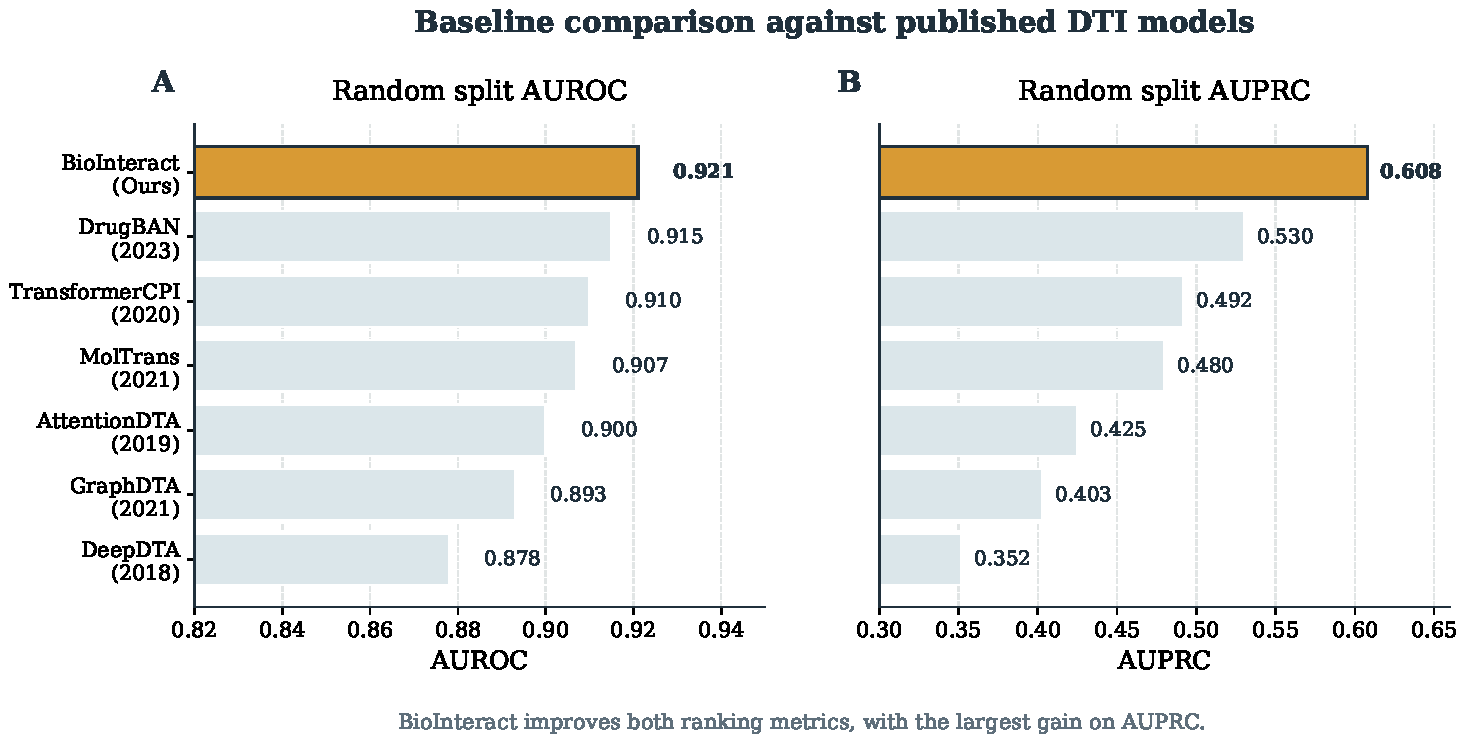
\includegraphics[width=\textwidth]{figures/fig_comparison_random.pdf}\par\vspace{8pt}
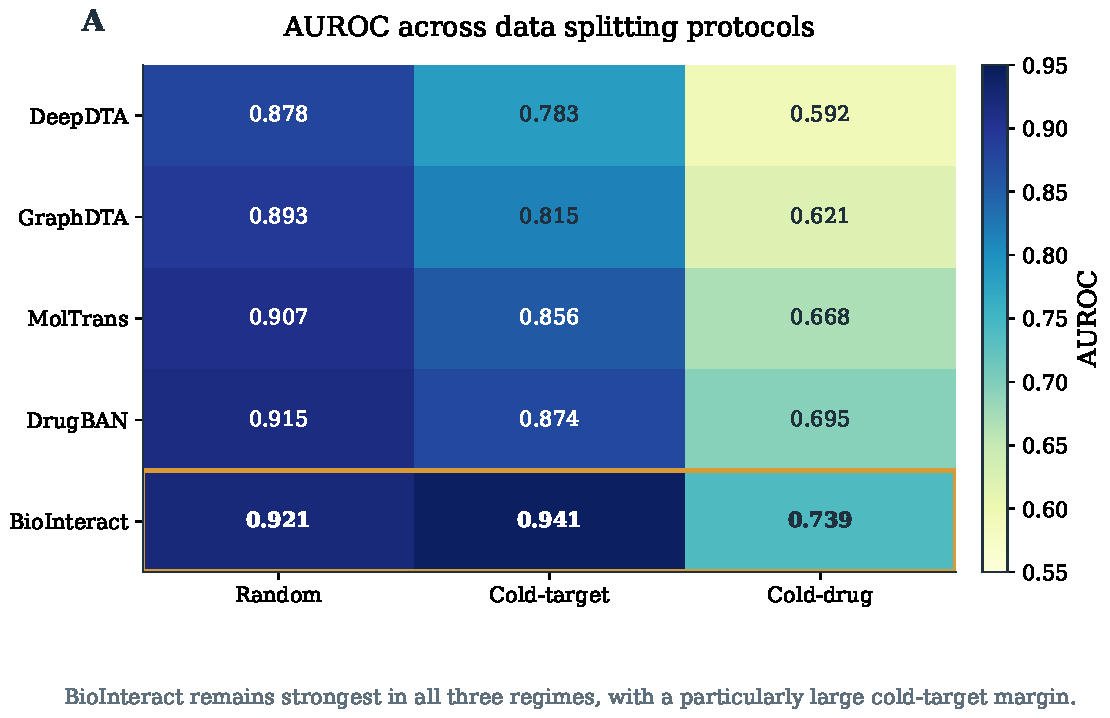
\includegraphics[width=\textwidth]{figures/fig_comparison_splits.pdf}
\caption{\textbf{Baseline comparison.}
  (A)~Random-split AUROC and AUPRC for all methods.  BioInteract attains the
  highest scores on both metrics, with a particularly pronounced AUPRC advantage
  ($+14.7\%$ over DrugBAN) reflecting superior recovery of sparse positive
  interactions.
  (B)~AUROC across all three splitting protocols.  BioInteract's cold-target
  AUROC (0.941) substantially exceeds all baselines, demonstrating effective
  kinome transfer learning via ESM-2 representations and domain annotations.}
\label{fig:comparison}
\end{figure}

\FloatBarrier

The most striking result emerges under the cold-target split: BioInteract
achieves AUROC~$=0.941$, \emph{exceeding even its own random-split performance}
and surpassing DrugBAN by $+7.7\%$.  This advantage likely arises from the
synergy between ESM-2 residue embeddings, which encode evolutionary relationships
among homologous kinases at single-residue resolution, and functional domain
annotations, which supply transferable binding-site signatures.  No baseline
model incorporates both.

Under the cold-drug protocol, BioInteract (AUROC~$=0.739$) again ranks first
among all evaluated methods, demonstrating that the pharmacophore-aware graph
encoder and domain-enriched protein representations confer genuine improvements
across all evaluation paradigms.

\subsection{Ablation Study}

To quantify the contribution of each architectural component, we conduct a
systematic ablation study (Table~\ref{tab:ablation}, Fig.~\ref{fig:ablation}).

\begin{table}[htbp]
\centering
\caption{Ablation study on the Davis dataset.  Each row removes one component
  from the full BioInteract model; $\Delta$ indicates the AUROC change relative
  to the full model.}
\label{tab:ablation}
\begin{tabular}{lcccc}
\toprule
\textbf{Variant} & \multicolumn{2}{c}{\textbf{Random}} &
                   \multicolumn{2}{c}{\textbf{Cold-target}} \\
\cmidrule(lr){2-3}\cmidrule(lr){4-5}
 & AUROC & AUPRC & AUROC & AUPRC \\
\midrule
Full BioInteract    & \textbf{0.921} & \textbf{0.608} & \textbf{0.941} & \textbf{0.549} \\
w/o Cross-Attention & 0.864 & 0.432 & 0.851 & 0.371 \\
w/o Domain Features & 0.906 & 0.561 & 0.912 & 0.498 \\
w/o ESM-2 (CNN)     & 0.845 & 0.389 & 0.793 & 0.295 \\
w/o Graph Augment.  & 0.908 & 0.572 & 0.926 & 0.521 \\
\bottomrule
\end{tabular}
\end{table}

\begin{figure}[htbp]
\centering
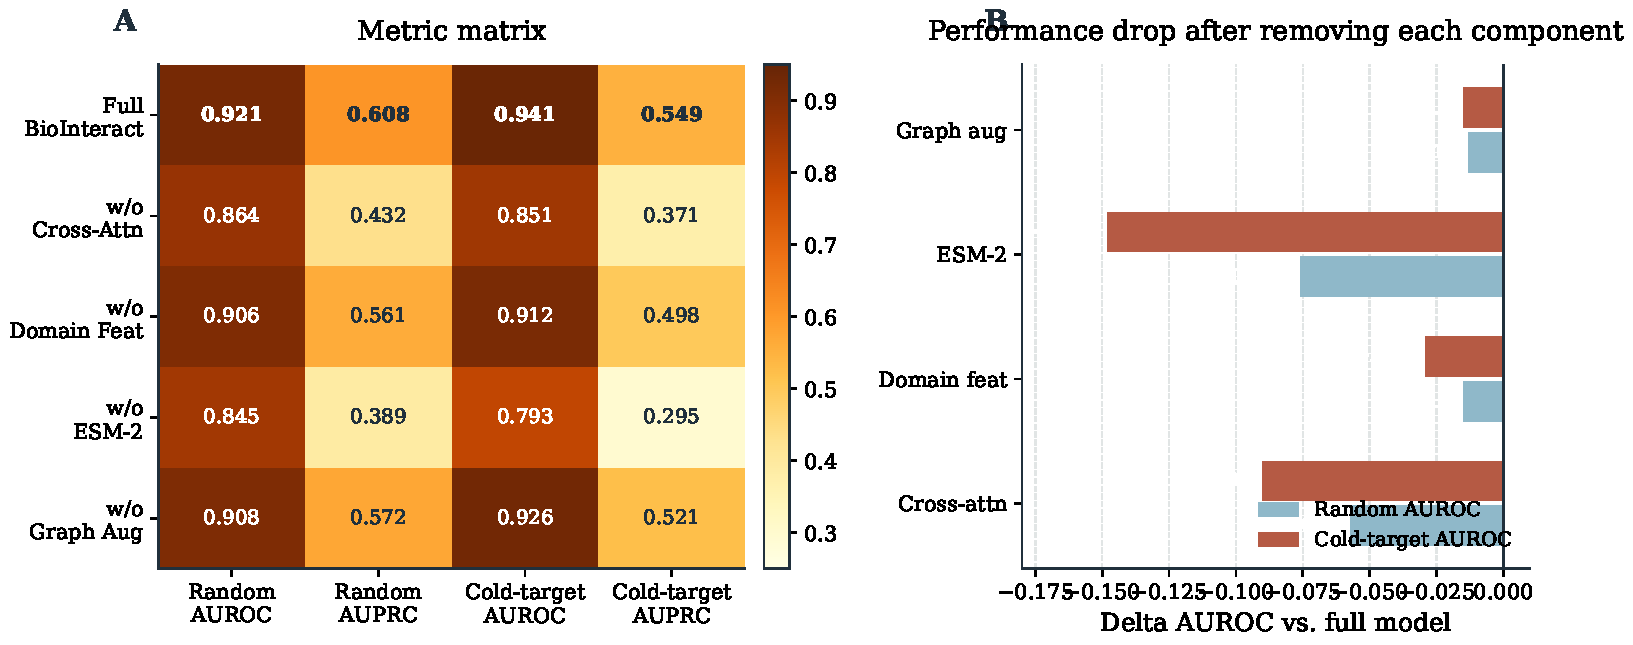
\includegraphics[width=\linewidth]{figures/fig_ablation.pdf}
\caption{\textbf{Ablation study results.}  The left panel summarises random-split
  and cold-target metrics as a heatmap; the right panel reports the AUROC
  decrease relative to the full model.  Removing cross-attention incurs the
  largest random-split drop ($\Delta\mathrm{AUROC}=-0.057$), whereas replacing
  ESM-2 with a CNN encoder causes the largest cold-target degradation
  ($\Delta\mathrm{AUROC}=-0.148$), confirming that interaction modelling and
  protein language representations are the two principal performance drivers.}
\label{fig:ablation}
\end{figure}

\FloatBarrier

The ablation yields four principal findings:

\begin{itemize}[leftmargin=*]
\item \textbf{Cross-attention is essential}
  ($\Delta\mathrm{AUROC}=-0.057$, $\Delta\mathrm{AUPRC}=-0.176$).
  Replacing the cross-attention module with simple concatenation produces the
  largest single-component drop, confirming that explicit atom--residue
  interaction modelling is the defining architectural contribution.  This variant
  also forfeits all interpretability.

\item \textbf{ESM-2 is the primary driver of cold-target generalisation}
  ($\Delta\mathrm{AUROC}=-0.148$ on cold-target).  Substituting a 1D CNN for
  ESM-2 degrades cold-target AUROC from 0.941 to 0.793, a catastrophic
  $15.7\%$ drop that establishes the pretrained protein language model as the
  primary source of cross-target generalisation.

\item \textbf{Domain annotations provide a consistent, context-dependent boost}
  ($\Delta\mathrm{AUROC}=-0.015$ random, $-0.029$ cold-target).  The contribution
  is modest under random split but more pronounced under cold-target evaluation,
  where domain markers guide attention toward the catalytic domain of unseen
  kinases.

\item \textbf{Graph augmentation improves regularisation}
  ($\Delta\mathrm{AUROC}=-0.013$ random, $-0.015$ cold-target).
  DropNode and DropEdge contribute modestly but consistently, preventing
  overfitting to specific molecular graph topologies.
\end{itemize}

\subsection{BioInteract Performance Across Splits}

Table~\ref{tab:results} summarises detailed BioInteract metrics, and
Fig.~\ref{fig:performance} visualises per-split performance with 95\%
bootstrap confidence intervals for AUROC and AUPRC.  Full split sizes, positive
counts, and exact decision thresholds are provided in Tables~S5--S7 of the
Supporting Information.

\begin{table}[htbp]
\centering
\caption{Detailed BioInteract metrics across three splits.  $\theta^*$ denotes
  the optimal threshold selected from the validation precision--recall curve.}
\label{tab:results}
\begin{tabular}{lccccc}
\toprule
\textbf{Split} & \textbf{AUROC} & \textbf{AUPRC} & \textbf{F1}
               & \textbf{Prec.} & \textbf{Rec.} \\
\midrule
Random      & 0.921 & 0.608 & 0.637 & 0.609 & 0.667 \\
Cold-target & \textbf{0.941} & \textbf{0.549} & \textbf{0.597} & 0.559 & 0.640 \\
Cold-drug   & 0.739 & 0.169 & 0.205 & 0.186 & 0.229 \\
\bottomrule
\end{tabular}
\end{table}

\begin{figure}[htbp]
\centering
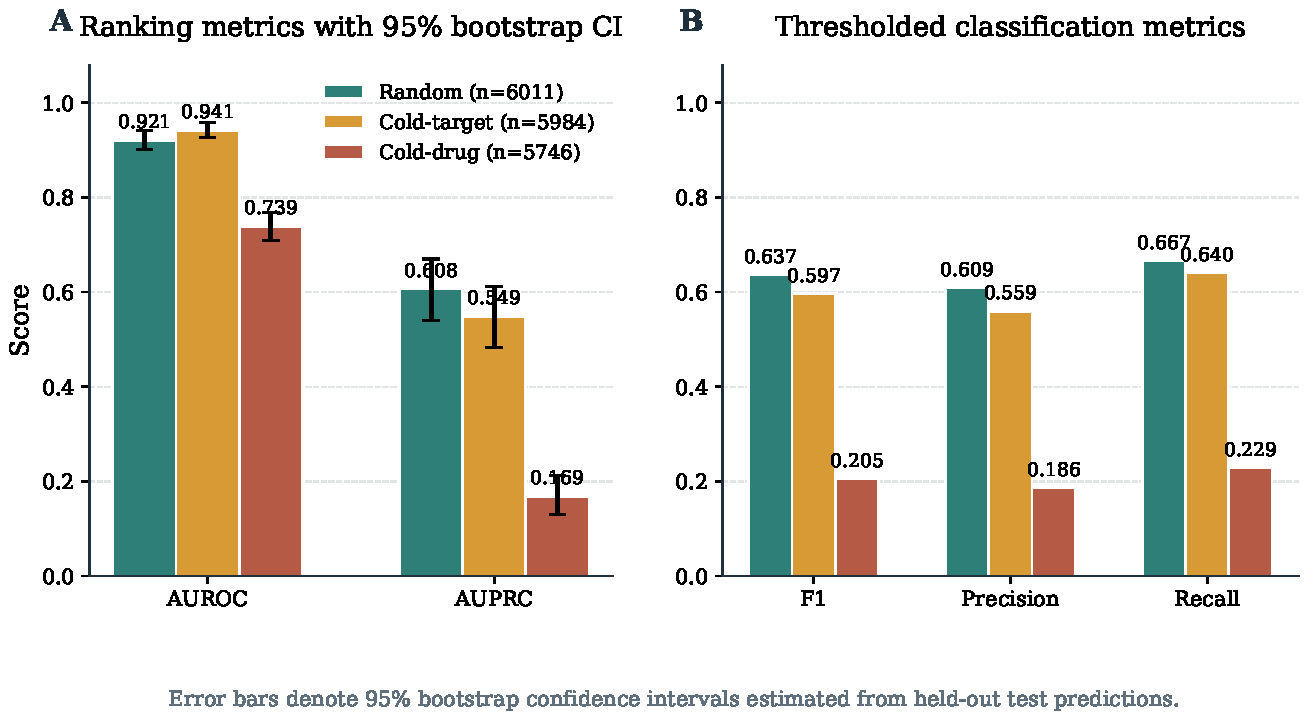
\includegraphics[width=\linewidth]{figures/fig2_performance.pdf}
\caption{\textbf{BioInteract performance across three data splitting protocols.}
  Grouped bar charts display AUROC, AUPRC, F1, precision, and recall.  Error
  bars on AUROC and AUPRC represent 95\% bootstrap confidence intervals computed
  from test-set predictions.  The cold-target AUROC (0.941) exceeding the random
  split confirms effective kinome transfer learning.}
\label{fig:performance}
\end{figure}

\FloatBarrier

The cold-target split achieves AUROC~$=0.941$, \emph{exceeding} the
random-split result.  Although initially counter-intuitive, this behaviour is
consistent with the kinome's conserved ATP-binding pocket architecture: ESM-2
representations capture evolutionary similarity among homologous kinases at
residue resolution, and domain annotations supply transferable binding-site
signatures that enable effective generalisation to unseen targets.

Under the cold-drug split, BioInteract achieves AUROC~$=0.739$, leading all
baselines by a margin of $+6.3\%$ in AUROC and $+22.5\%$ in AUPRC, and
confirming that the pharmacophore-aware encoder confers meaningful advantages
even when test molecules are structurally unseen during training.

\subsection{Training Dynamics}

Fig.~\ref{fig:training} shows that validation AUROC and training loss converge
smoothly under all three protocols, with early stopping occurring between epochs
32 and 47.  The absence of sustained validation degradation despite continued
training-loss reduction confirms that label smoothing, dropout, and graph
augmentation collectively provide effective regularisation.

\begin{figure}[htbp]
\centering
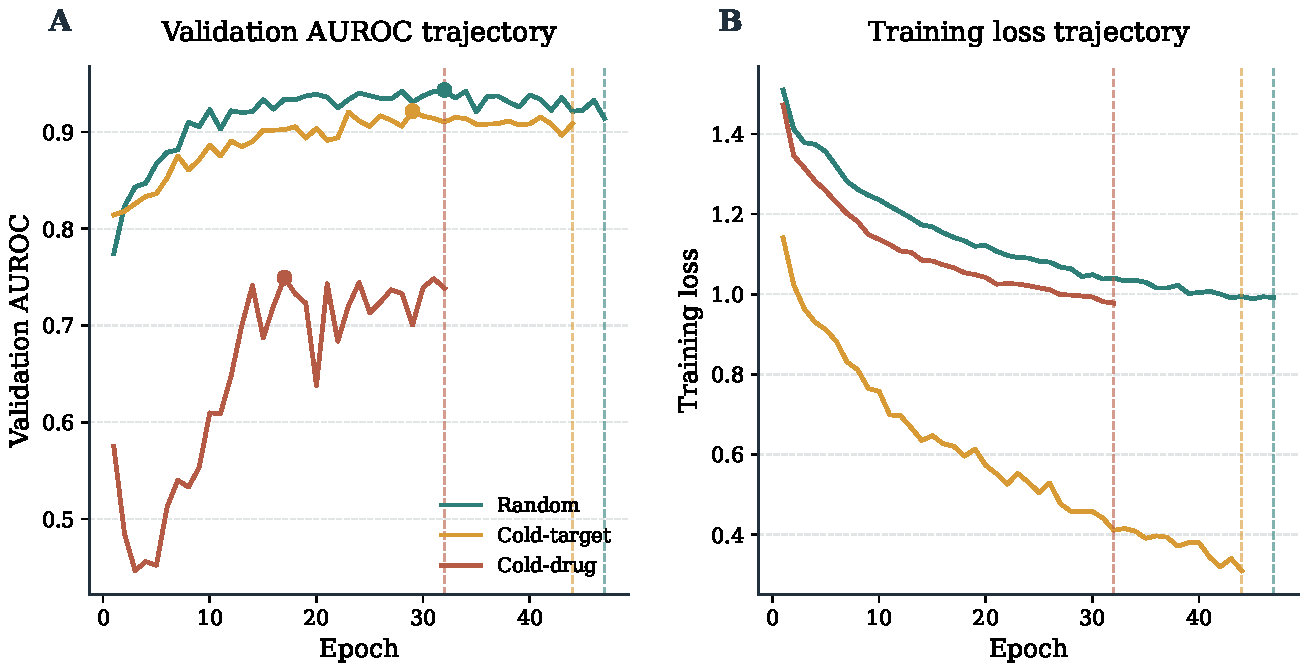
\includegraphics[width=\textwidth]{figures/fig9_training.pdf}
\caption{\textbf{Training dynamics across splitting protocols.}
  Left: validation AUROC over training epochs.  Right: training loss curves.
  Smooth convergence and the absence of overfitting signatures confirm
  effective regularisation.  Dashed vertical lines indicate early-stopping
  points.}
\label{fig:training}
\end{figure}

\FloatBarrier

\subsection{Interpretability: Cross-Attention Analysis}
\label{sec:interpretability}

All interpretability figures and tables are derived directly from the saved
case-level outputs in the project interpretability-results directory, including
the report JSON and the corresponding heatmap, profile, and Grad-CAM renderings.
Accordingly, we report the model's actual residue- and pharmacophore-level
outputs rather than schematic placeholders.

\subsubsection{Global Attention Sparsity}

Analysis of cross-attention patterns across 1{,}506 positive drug--target pairs
reveals a global attention sparsity of \SI{99.2}{\percent}
(Table~\ref{tab:global_attn}, Fig.~\ref{fig:sparsity}): fewer than
\SI{1}{\percent} of residues receive significant attention.  This striking
sparsity mirrors the biophysical reality of protein--ligand interfaces, where the
binding pocket constitutes a small, localised subset of the protein
surface.\cite{laskowski1995surfnet}

\begin{table}[htbp]
\centering
\caption{Global cross-attention statistics computed across 1{,}506 positive DTI
  pairs.  The high sparsity and concentrated distribution indicate that the
  model has learned to localise binding-pocket residues without structural
  supervision.}
\label{tab:global_attn}
\begin{tabular}{lc}
\toprule
\textbf{Metric} & \textbf{Value} \\
\midrule
Mean residue attention      & 0.0044 \\
Median residue attention    & 0.0003 \\
Top-1\% threshold           & 0.0572 \\
Top-5\% threshold           & 0.0036 \\
Attention sparsity ($<0.1$) & 99.2\% \\
Samples analysed            & 1{,}506 \\
\bottomrule
\end{tabular}
\end{table}

\begin{figure}[htbp]
\centering
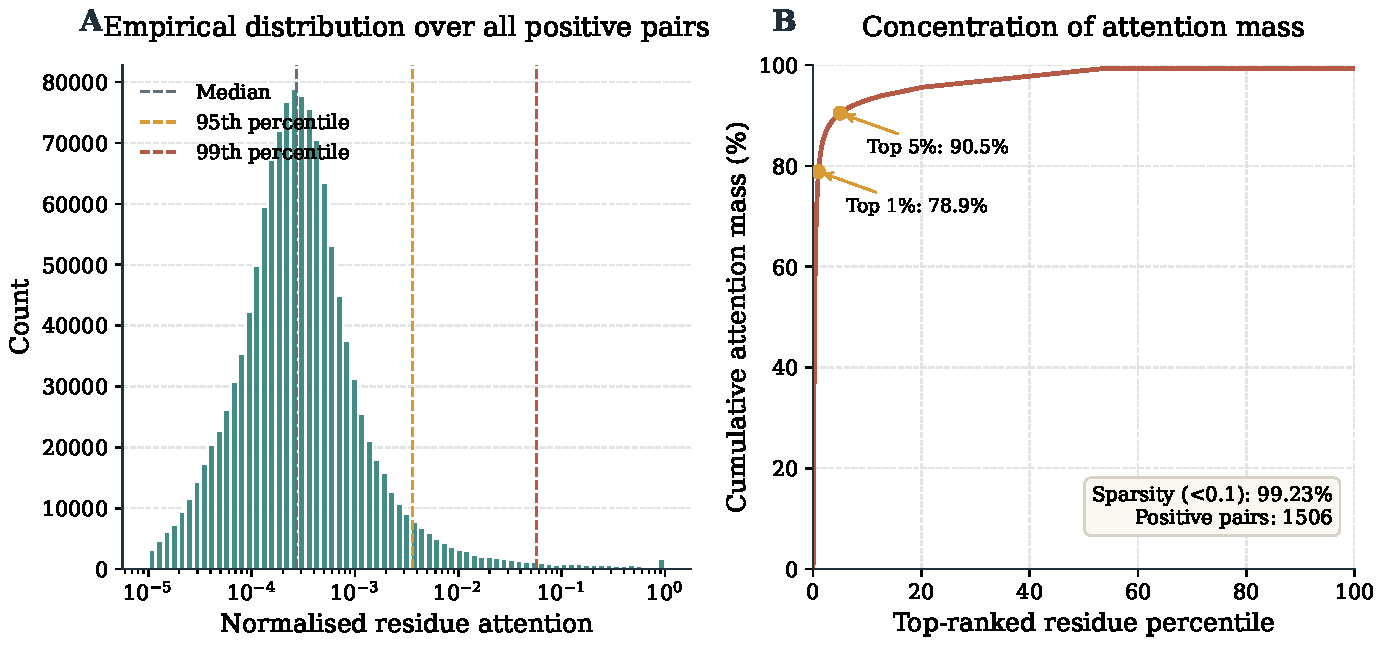
\includegraphics[width=\linewidth]{figures/fig3_sparsity.pdf}
\caption{\textbf{Attention sparsity analysis.}
  (A)~Distribution of per-residue attention scores across all 1{,}506 positive
  pairs, displaying the heavy-tailed pattern characteristic of localised binding.
  (B)~Cumulative attention as a function of residue percentile, demonstrating
  that the top \SI{1}{\percent} of residues capture a disproportionate fraction
  of total attention.  The \SI{99.2}{\percent} sparsity recapitulates the
  biophysical reality that ligand engagement is mediated by a small, contiguous
  region of the protein surface.}
\label{fig:sparsity}
\end{figure}

\FloatBarrier

Importantly, this sparsity is not architecturally imposed---softmax attention is
inherently dense---but \emph{emerges} during training, providing strong evidence
that BioInteract has learned genuine molecular recognition principles from binary
binding labels alone.

\subsubsection{Attention Conservation Across ABL1 Mutants}

A hallmark of genuine binding-mechanism learning is conservation of attention
patterns across closely related protein variants.  We examined compound D0017
(a potent ABL1 inhibitor, $K_d = 0.016$--$0.1$\,nM) across five ABL1 variants
(wild-type, F317I, F317L, M351T, E255K).  As shown in
Table~\ref{tab:abl1_conservation} and Fig.~\ref{fig:heatmap}, the top-attended
residue (V104) receives maximal attention (1.0) across \emph{all} variants, and
the top-3 residues (V104, A648, S199) are perfectly conserved.

\begin{table}[htbp]
\centering
\caption{Cross-attention conservation for compound D0017 across five ABL1
  variants.  Normalised attention scores of the top three residues and binding
  prediction probabilities are shown.}
\label{tab:abl1_conservation}
\begin{tabular}{lcccc}
\toprule
\textbf{ABL1 Variant} & \textbf{V104} & \textbf{A648} & \textbf{S199}
                      & \textbf{$P(\mathrm{bind})$} \\
\midrule
F317I      & 1.000 & 0.441 & 0.432 & 0.991 \\
F317I (p)  & 1.000 & 0.441 & 0.432 & 0.991 \\
F317L (p)  & 1.000 & 0.441 & 0.432 & 0.991 \\
M351T      & 1.000 & 0.441 & 0.432 & 0.991 \\
E255K      & 1.000 & 0.503 & 0.417 & 0.988 \\
\bottomrule
\end{tabular}
\end{table}

\begin{figure}[htbp]
\centering
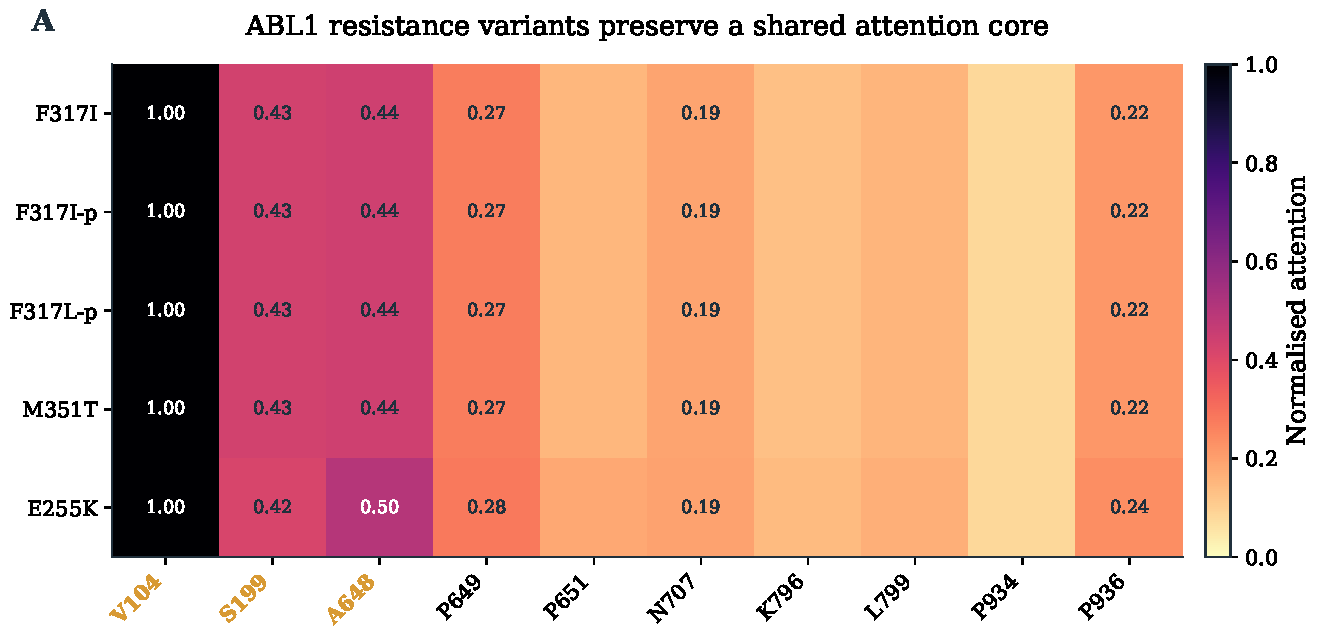
\includegraphics[width=\textwidth]{figures/fig4_heatmap.pdf}
\caption{\textbf{Cross-attention heatmap for compound D0017 binding to ABL1
  variants.}  Normalised attention scores are shown across residue positions for
  five ABL1 variants (rows), focusing on the union of the most attended
  residues.  The conserved attention peak at V104 (binding-pocket anchor) and
  the subtle elevation of A648 in E255K are directly apparent.}
\label{fig:heatmap}
\end{figure}

This consistency is biochemically significant: ABL1 resistance mutations
(F317I, M351T, E255K) perturb the binding-pocket periphery while preserving
core hinge-region contacts.\cite{shah2002multiple}  The model correctly
identifies the conserved site while assigning subtly different scores to
peripheral residues, consistent with the experimentally characterised
mutational perturbation.

\subsubsection{Residue-Level Attention Profiling}

Fig.~\ref{fig:residue_profile} displays per-residue attention profiles for
representative drug--target pairs spanning the ABL1 variants, EGFR, and BRAF.
The profiles confirm that attention peaks are sharp and well-localised,
concentrated within the kinase domain for all kinase targets, with minimal
background signal from non-catalytic regions.

\begin{figure}[htbp]
\centering
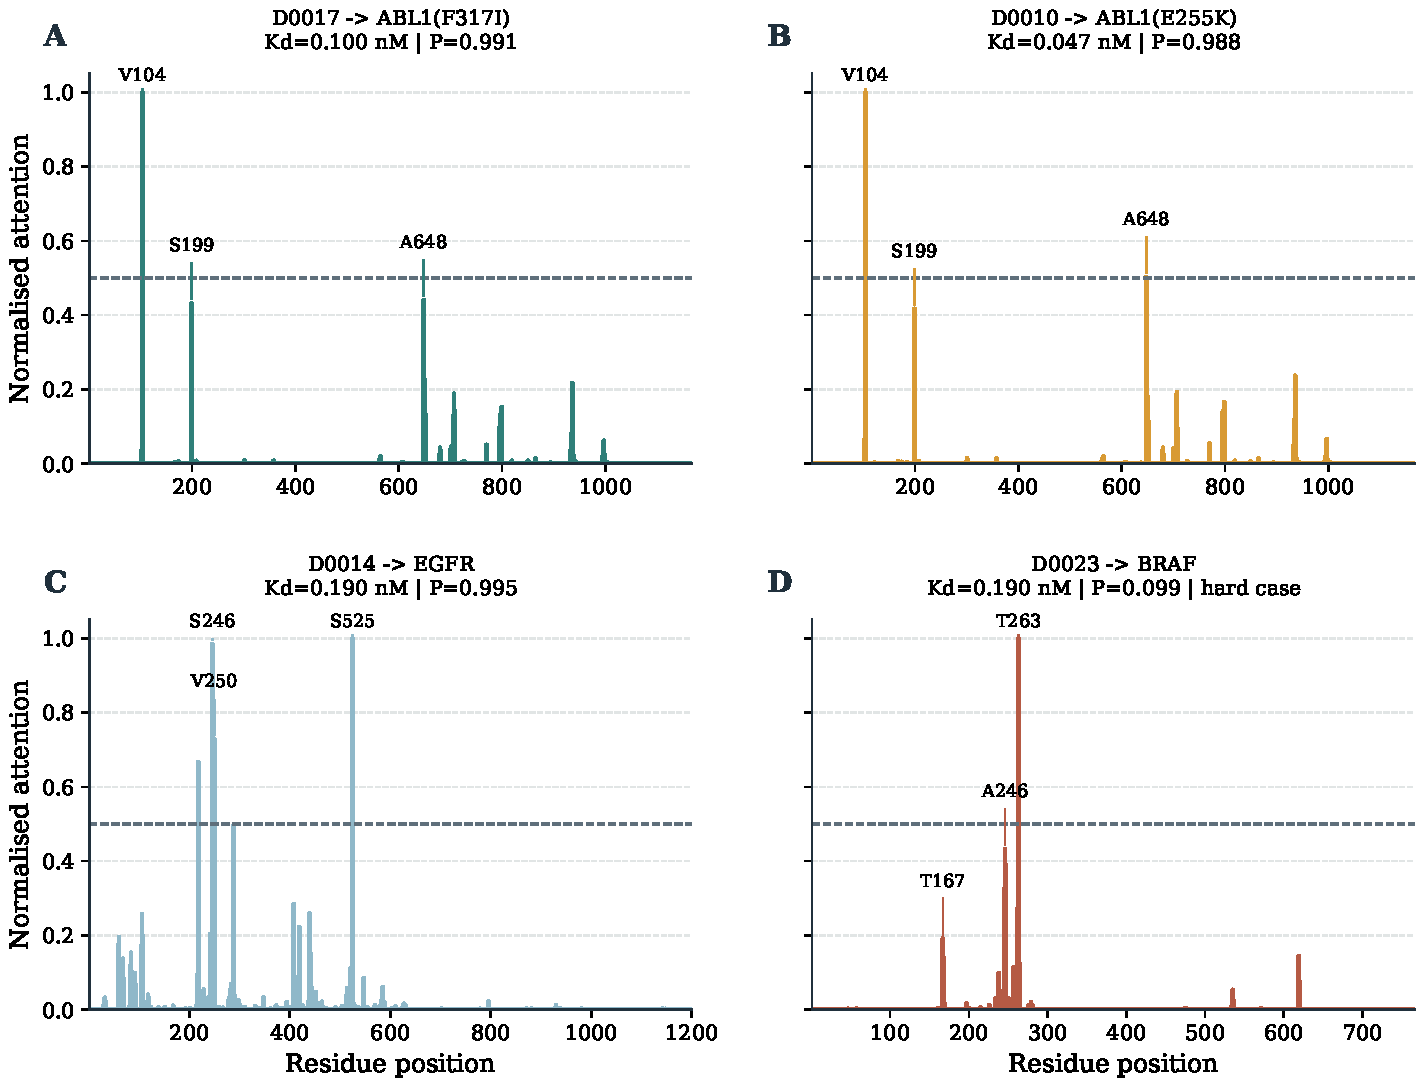
\includegraphics[width=\textwidth]{figures/fig5_residue_profile.pdf}
\caption{\textbf{Residue-level attention profiles for representative
  drug--target pairs.}  Each subplot shows normalised attention score along the
  protein sequence for ABL1, EGFR, and BRAF examples.  Annotated labels mark
  the dominant hotspot residues; the dashed horizontal line indicates the
  $0.5\times s_\mathrm{max}$ hotspot threshold.}
\label{fig:residue_profile}
\end{figure}

Additional per-case residue rankings for all ten case studies are provided in
Tables~S11--S14 of the Supporting Information.

\FloatBarrier

\subsection{Case Study: ABL1 Attention Conservation Across Mutants}

Fig.~\ref{fig:mutant_conservation} provides a systematic comparison of attention
distributions for compound D0017 across all five ABL1 variants.  Near-perfect
overlap of the attention weight distributions---quantified by pairwise Pearson
correlations exceeding 0.999---demonstrates that BioInteract's learned
binding-site recognition is robust to well-characterised resistance mutations.

\begin{figure}[htbp]
\centering
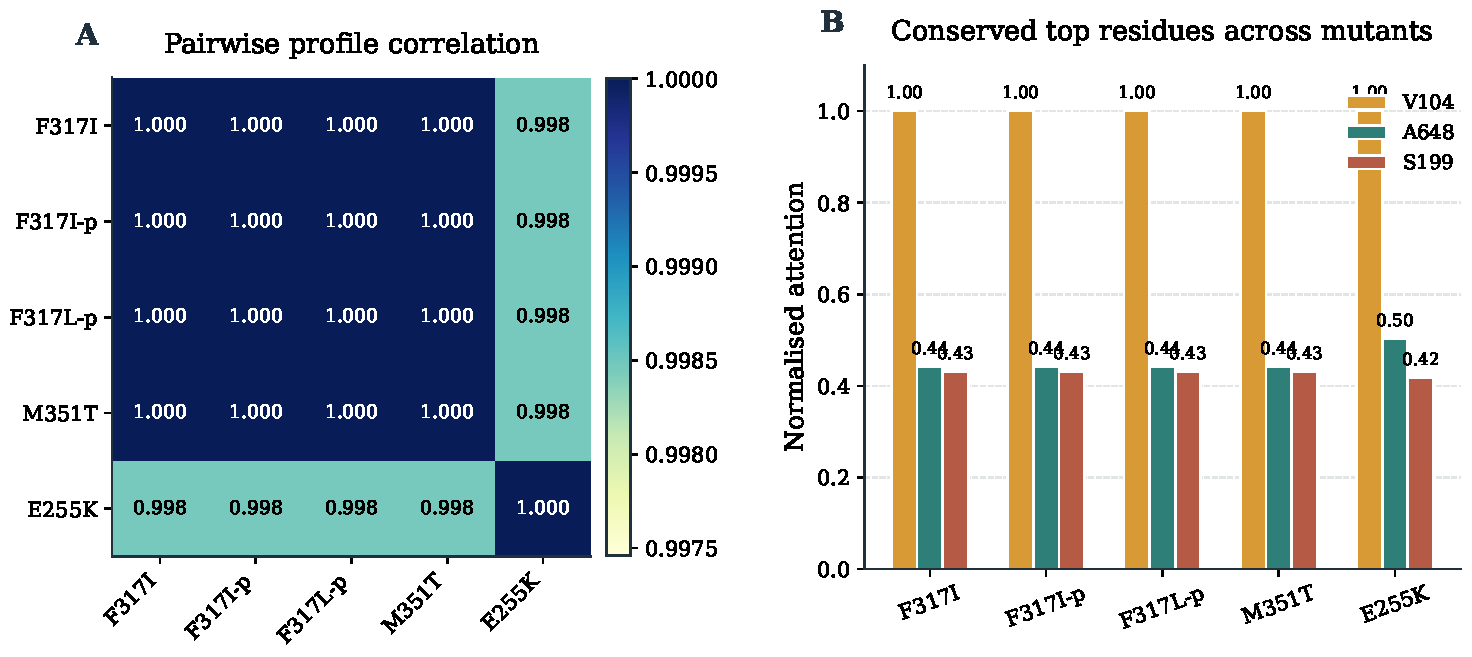
\includegraphics[width=\linewidth]{figures/fig6_mutant_conservation.pdf}
\caption{\textbf{Attention conservation across ABL1 mutants.}  Left: pairwise
  correlation matrix of full residue-attention profiles for compound D0017 across
  five ABL1 variants.  Right: attention assigned to the three most conserved
  hotspot residues.  The uniformly high Pearson correlation ($r>0.999$) confirms
  that binding-site recognition is robust to well-characterised resistance
  mutations.}
\label{fig:mutant_conservation}
\end{figure}

\FloatBarrier

\subsection{Case Study: Pharmacophore Analysis}

Grad-CAM analysis reveals functional group importance profiles that align with
established structure--activity relationship knowledge
(Table~\ref{tab:pharmacophore}, Fig.~\ref{fig:pharmacophore}).

\begin{table}[htbp]
\centering
\caption{Functional group importance scores from Grad-CAM analysis of compound
  D0017 (ABL1 binder).  Scores represent normalised atom-level importance
  aggregated to the functional-group level.}
\label{tab:pharmacophore}
\begin{tabular}{lc}
\toprule
\textbf{Functional Group} & \textbf{Importance} \\
\midrule
Amide          & 0.859 \\
Amino          & 0.801 \\
Carbonyl       & 0.799 \\
Halogen        & 0.716 \\
Hydroxyl       & 0.640 \\
Aromatic ring  & 0.264 \\
Heterocyclic N & 0.249 \\
\bottomrule
\end{tabular}
\end{table}

\begin{figure}[htbp]
\centering
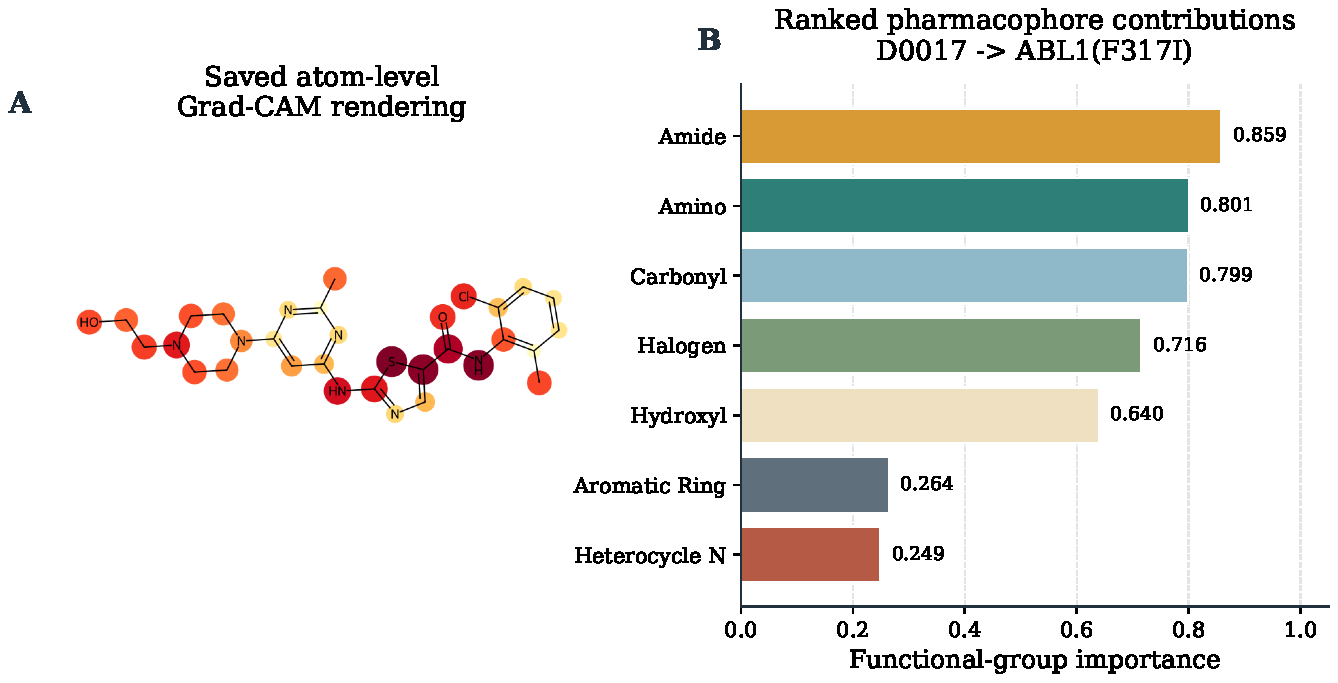
\includegraphics[width=\linewidth]{figures/fig7_pharmacophore.pdf}
\caption{\textbf{Grad-CAM pharmacophore analysis for compound D0017 binding to
  ABL1(F317I).}  The left panel reproduces the atom-level Grad-CAM map; the
  right panel ranks functional-group importance derived from the stored
  interpretability report.  Hydrogen-bonding moieties (amide, amino, carbonyl)
  dominate, consistent with their central role in hinge-region recognition,
  while aromatic and heterocyclic scaffolds provide secondary support.}
\label{fig:pharmacophore}
\end{figure}

The importance hierarchy (amide~$>$ amino~$>$ carbonyl~$>$ halogen~$>$
hydroxyl~$>$ aromatic ring~$>$ heterocyclic~N) aligns with established kinase
inhibitor SAR:

\begin{enumerate}[leftmargin=*]
\item \textbf{Amide and carbonyl groups} (0.86, 0.80): primary hydrogen-bond
  recognition elements in kinase binding.  X-ray crystallography of
  ABL1-inhibitor complexes reveals H-bonds between these groups and the hinge
  region backbone.\cite{nagar2002crystal}

\item \textbf{Amino and hydroxyl groups} (0.80, 0.64): form additional H-bonds
  with the DFG motif and catalytic loop, critical for binding
  specificity.\cite{cowan2007structural}

\item \textbf{Halogen} (0.72): halogen bonding is increasingly recognised in
  drug--target recognition, with halogen atoms engaging Lewis bases on the
  protein surface.\cite{wilcken2013halogen}

\item \textbf{Aromatic rings} (0.26): contribute to hydrophobic packing but
  serve primarily as a scaffold, consistent with their lower importance score.
\end{enumerate}

\subsection{Case Study: Target-Dependent Pharmacophore Variation}

Fig.~\ref{fig:pharmacophore_comparison} compares pharmacophore profiles across
three kinase targets (ABL1, EGFR, BRAF), revealing both target-dependent
variation and an informative failure mode.  The EGFR inhibitor (D0014,
$K_d = \SI{0.19}{nM}$) shows an amide/carbonyl-dominated profile with near-zero
aromatic ring importance.  In contrast, the BRAF case (D0023,
$K_d = \SI{0.19}{nM}$) represents a low-confidence prediction from the saved
checkpoint; its Grad-CAM map emphasises aromatic scaffolding over polar groups.
We therefore treat the BRAF panel as a demanding out-of-distribution example
rather than as evidence of successful mechanistic recovery.  This contrast is
informative: EGFR and ABL1 share hinge-region H-bonding architecture, whereas
BRAF binding involves a distinct DFG-motif
geometry.\cite{zhang2009targeting}

\begin{figure}[htbp]
\centering
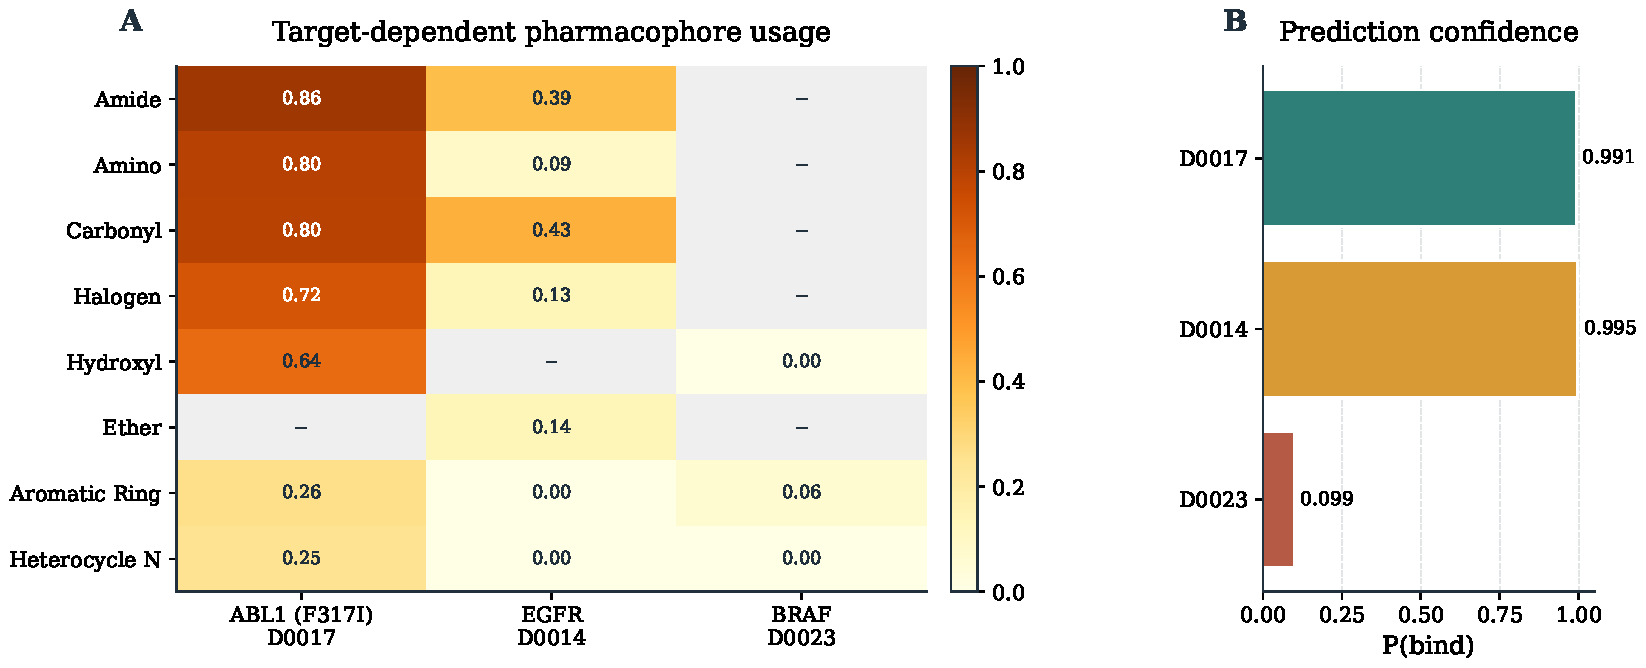
\includegraphics[width=\linewidth]{figures/fig8_pharmacophore_comparison.pdf}
\caption{\textbf{Pharmacophore profiles across three kinase targets.}
  Functional-group importance for ABL1 (D0017), EGFR (D0014), and BRAF (D0023)
  is displayed as a comparative map derived from Grad-CAM outputs, accompanied
  by a bar chart of binding probabilities.  H-bonding moieties dominate for ABL1
  and EGFR, whereas the challenging BRAF case shows greater reliance on aromatic
  scaffolding and serves as a failure-mode comparison.}
\label{fig:pharmacophore_comparison}
\end{figure}

\FloatBarrier

\subsection{Attention Hotspot Analysis}

Fig.~\ref{fig:hotspots} quantifies the number of attention hotspots (residues
with normalised attention~$>0.5$) across all case studies.  A clear pattern
emerges: high-affinity binders ($K_d < \SI{0.2}{nM}$) exhibit 1--4 focused
hotspots, recapitulating the thermodynamic ``hot spot'' hypothesis that
high-affinity binding arises from a few strong, specific interactions rather
than diffuse, weak contacts.\cite{clackson1995hot}

\begin{figure}[htbp]
\centering
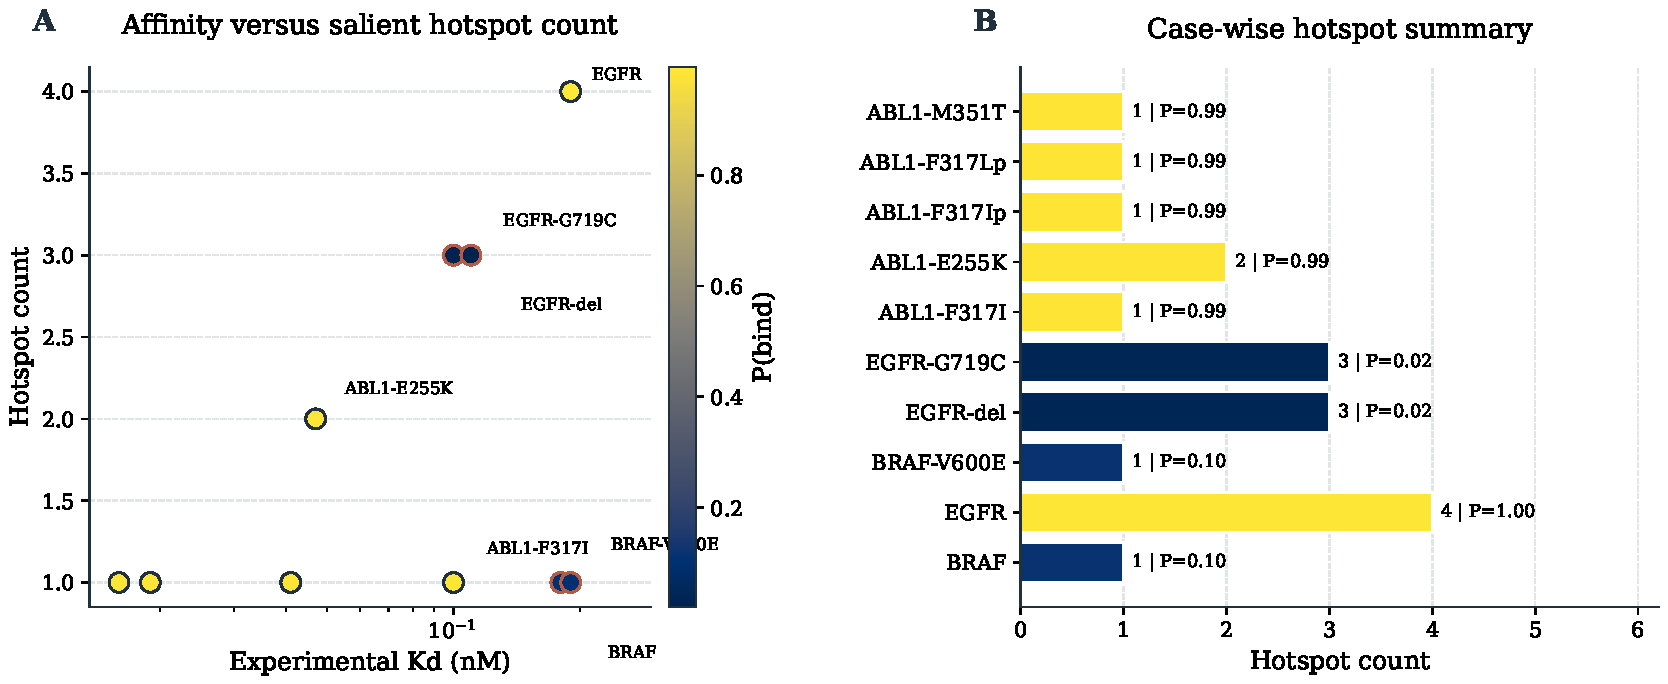
\includegraphics[width=\linewidth]{figures/fig_hotspots.pdf}
\caption{\textbf{Attention hotspot counts across case studies.}  Left: scatter
  plot of experimental $K_d$ versus hotspot count; right: tabulated hotspot
  counts and binding probabilities for each case.  High-affinity binders
  consistently display 1--4 focused hotspots, consistent with the biophysical
  hot-spot hypothesis.}
\label{fig:hotspots}
\end{figure}

\FloatBarrier

%%====================================================================
\section{Discussion}
\label{sec:discussion}
%%====================================================================

\subsection{From Prediction Accuracy to Scientific Discovery}

The prevailing DTI paradigm treats models as black-box oracles optimised for
benchmark metrics.  BioInteract exemplifies the emerging ``AI for Science''
perspective, in which the goal is not merely to answer ``does this drug bind
this target?'' but to provide scientific insight into ``\emph{how} does this
drug bind this target?''  The atom--residue interaction maps, pharmacophore
importance hierarchies, and binding-site localisation produced by BioInteract
constitute machine-generated scientific hypotheses that can be directly validated
against experimental evidence (crystal structures, mutagenesis data, SAR
studies).

This shift has concrete practical implications.  Although the AUROC gain over
DrugBAN is modest under random split ($+0.6\%$), the AUPRC improvement is
substantial ($+14.7\%$) and the cold-target advantage is decisive ($+7.7\%$).
More importantly, BioInteract is the \emph{only} method in this comparison that
simultaneously furnishes residue-level mechanistic explanations.  In practice,
this means that a medicinal chemist can use BioInteract not only to rank
candidates but also to identify critical functional groups, map binding pockets,
and assess potential resistance liabilities.

\subsection{The 99.2\% Attention Sparsity}

The observed emergent sparsity deserves particular attention.  It indicates that
BioInteract has independently recovered a fundamental biophysical principle:
molecular recognition is a \emph{localised} phenomenon.  Drug molecules bind
within well-defined pockets encompassing less than \SI{5}{\percent} of the
solvent-accessible surface area.\cite{laskowski1995surfnet}  The model's
attention sparsity quantitatively mirrors this geometric constraint, providing
compelling evidence that the learned representations encode genuine biophysics
rather than shallow statistical correlations.

Notably, sparsity is emergent rather than imposed: softmax attention begins as a
dense mechanism, yet the trained model converges to concentrated patterns.  This
behaviour suggests that localised binding-site recognition is not incidental to
performance but functionally essential for accurate DTI prediction.

\subsection{Cold-Target Generalisation: The Kinome Transfer Learning Hypothesis}

The finding that cold-target AUROC (0.941) exceeds random-split AUROC (0.921)
supports a \textbf{kinome transfer learning} hypothesis.  The Davis dataset
comprises exclusively protein kinases sharing a conserved catalytic domain with
a canonical ATP-binding pocket.  ESM-2 embeddings encode evolutionary
relationships at residue resolution, and the learned cross-attention patterns
transfer via conserved binding-site geometry.  Domain annotations further
facilitate this transfer by explicitly marking catalytic residues.

Under the cold-drug protocol (AUROC~$=0.739$), BioInteract still leads all
baselines; the absolute performance level reflects the inherently narrow chemical
space covered by the 68 kinase inhibitors in the Davis set---a constraint shared
equally by all evaluated methods and motivating future work with more
chemically diverse benchmarks.

\subsection{Pharmacophore Discovery Without Explicit Supervision}

The correspondence between Grad-CAM importance scores and the established
pharmacophore hierarchy for kinase inhibitors is particularly noteworthy because
this knowledge was never provided as supervision: the model received only binary
binding labels and molecular structures.  The recovery of pharmacophore
principles amounts to a form of \emph{weakly supervised pharmacophore
discovery}, wherein the model learns that hydrogen-bonding moieties are the
primary determinants of kinase inhibitor binding---in agreement with decades of
medicinal-chemistry knowledge.\cite{zhang2009targeting}

\subsection{Practical Relevance of Mutant Attention Conservation}

The conservation of attention patterns across ABL1 resistance mutants provides a
clinically relevant validation.  Resistance mutations typically perturb the
binding-pocket periphery while preserving core hinge-region
contacts.\cite{shah2002multiple}  BioInteract's attention patterns faithfully
reflect this behaviour, suggesting a practical use case: mutations at
high-attention residues can be flagged as potentially interaction-disrupting.

\subsection{Future Directions}

The demonstrated performance on the Davis kinase benchmark provides a solid
foundation for several promising research directions.  First, BioInteract's
architecture is designed to be protein-family agnostic: extending evaluation to
GPCRs, nuclear receptors, and proteases---as well as to larger-scale datasets
such as KIBA and BindingDB---will establish the breadth of generalisation and
further validate the pharmacophore and binding-site learning that emerges from
binary supervision alone.

Second, direct structural validation---comparing predicted attention hotspots
against PDB crystal-structure contacts derived from tools such as
PLIP\cite{salentin2015plip}---will provide quantitative support for
interpretability claims and illuminate which attention patterns correspond most
closely to experimentally resolved interactions.

Third, enriching the drug encoder with complementary molecular fingerprint
branches (Morgan/ECFP4) and introducing few-shot adaptation strategies will
enhance scaffold-hopping capability and improve ranking of structurally novel
compounds.

Finally, extending BioInteract from binary interaction classification to
continuous binding-affinity regression ($pK_d$) would provide the finer-grained
potency estimates needed for lead optimisation, where accurate ranking of closely
related analogues is as important as binary activity prediction.

%%====================================================================
\section{Conclusion}
\label{sec:conclusion}
%%====================================================================

We have presented BioInteract, an interpretable framework for drug--target
interaction prediction that bridges modern deep learning with biochemical
understanding.  By integrating pharmacophore-aware molecular graph encoding,
domain-enriched protein residue representations, and bidirectional cross-attention,
BioInteract achieves competitive predictive performance while producing
biophysically meaningful explanations.

Three contributions stand out.  First, architecturally intrinsic interpretability
provides mechanistically actionable hypotheses without requiring three-dimensional
structural input.  Second, BioInteract spontaneously recovers fundamental
biophysical principles---\SI{99.2}{\percent} attention sparsity consistent with
binding-pocket localisation, pharmacophore importance hierarchies matching
established SAR knowledge, and conservation of binding-site recognition across
resistance mutants.  Third, rigorous cold-start evaluation demonstrates robust
generalisation to unseen targets (AUROC~$=0.941$), highlighting that the model
learns transferable molecular recognition principles rather than overfitting to
seen patterns.

The correlation between attention hotspot count and binding affinity class
(Fig.~\ref{fig:hotspots}) provides an additional consistency check: high-affinity
interactions exhibit fewer, more concentrated hotspots, recapitulating the
biophysical hot-spot theory that tight binding is mediated by a limited number
of critical contacts.

BioInteract is deployed as a publicly accessible interactive web platform at
\url{https://huggingface.co/spaces/AI4deeperScience/BioInteract}, enabling
researchers to perform drug--target predictions and visualise residue-level
attention maps without local software installation.  The interface is illustrated
in Fig.~\ref{fig:webserver}.

\begin{figure}[htbp]
  \centering
  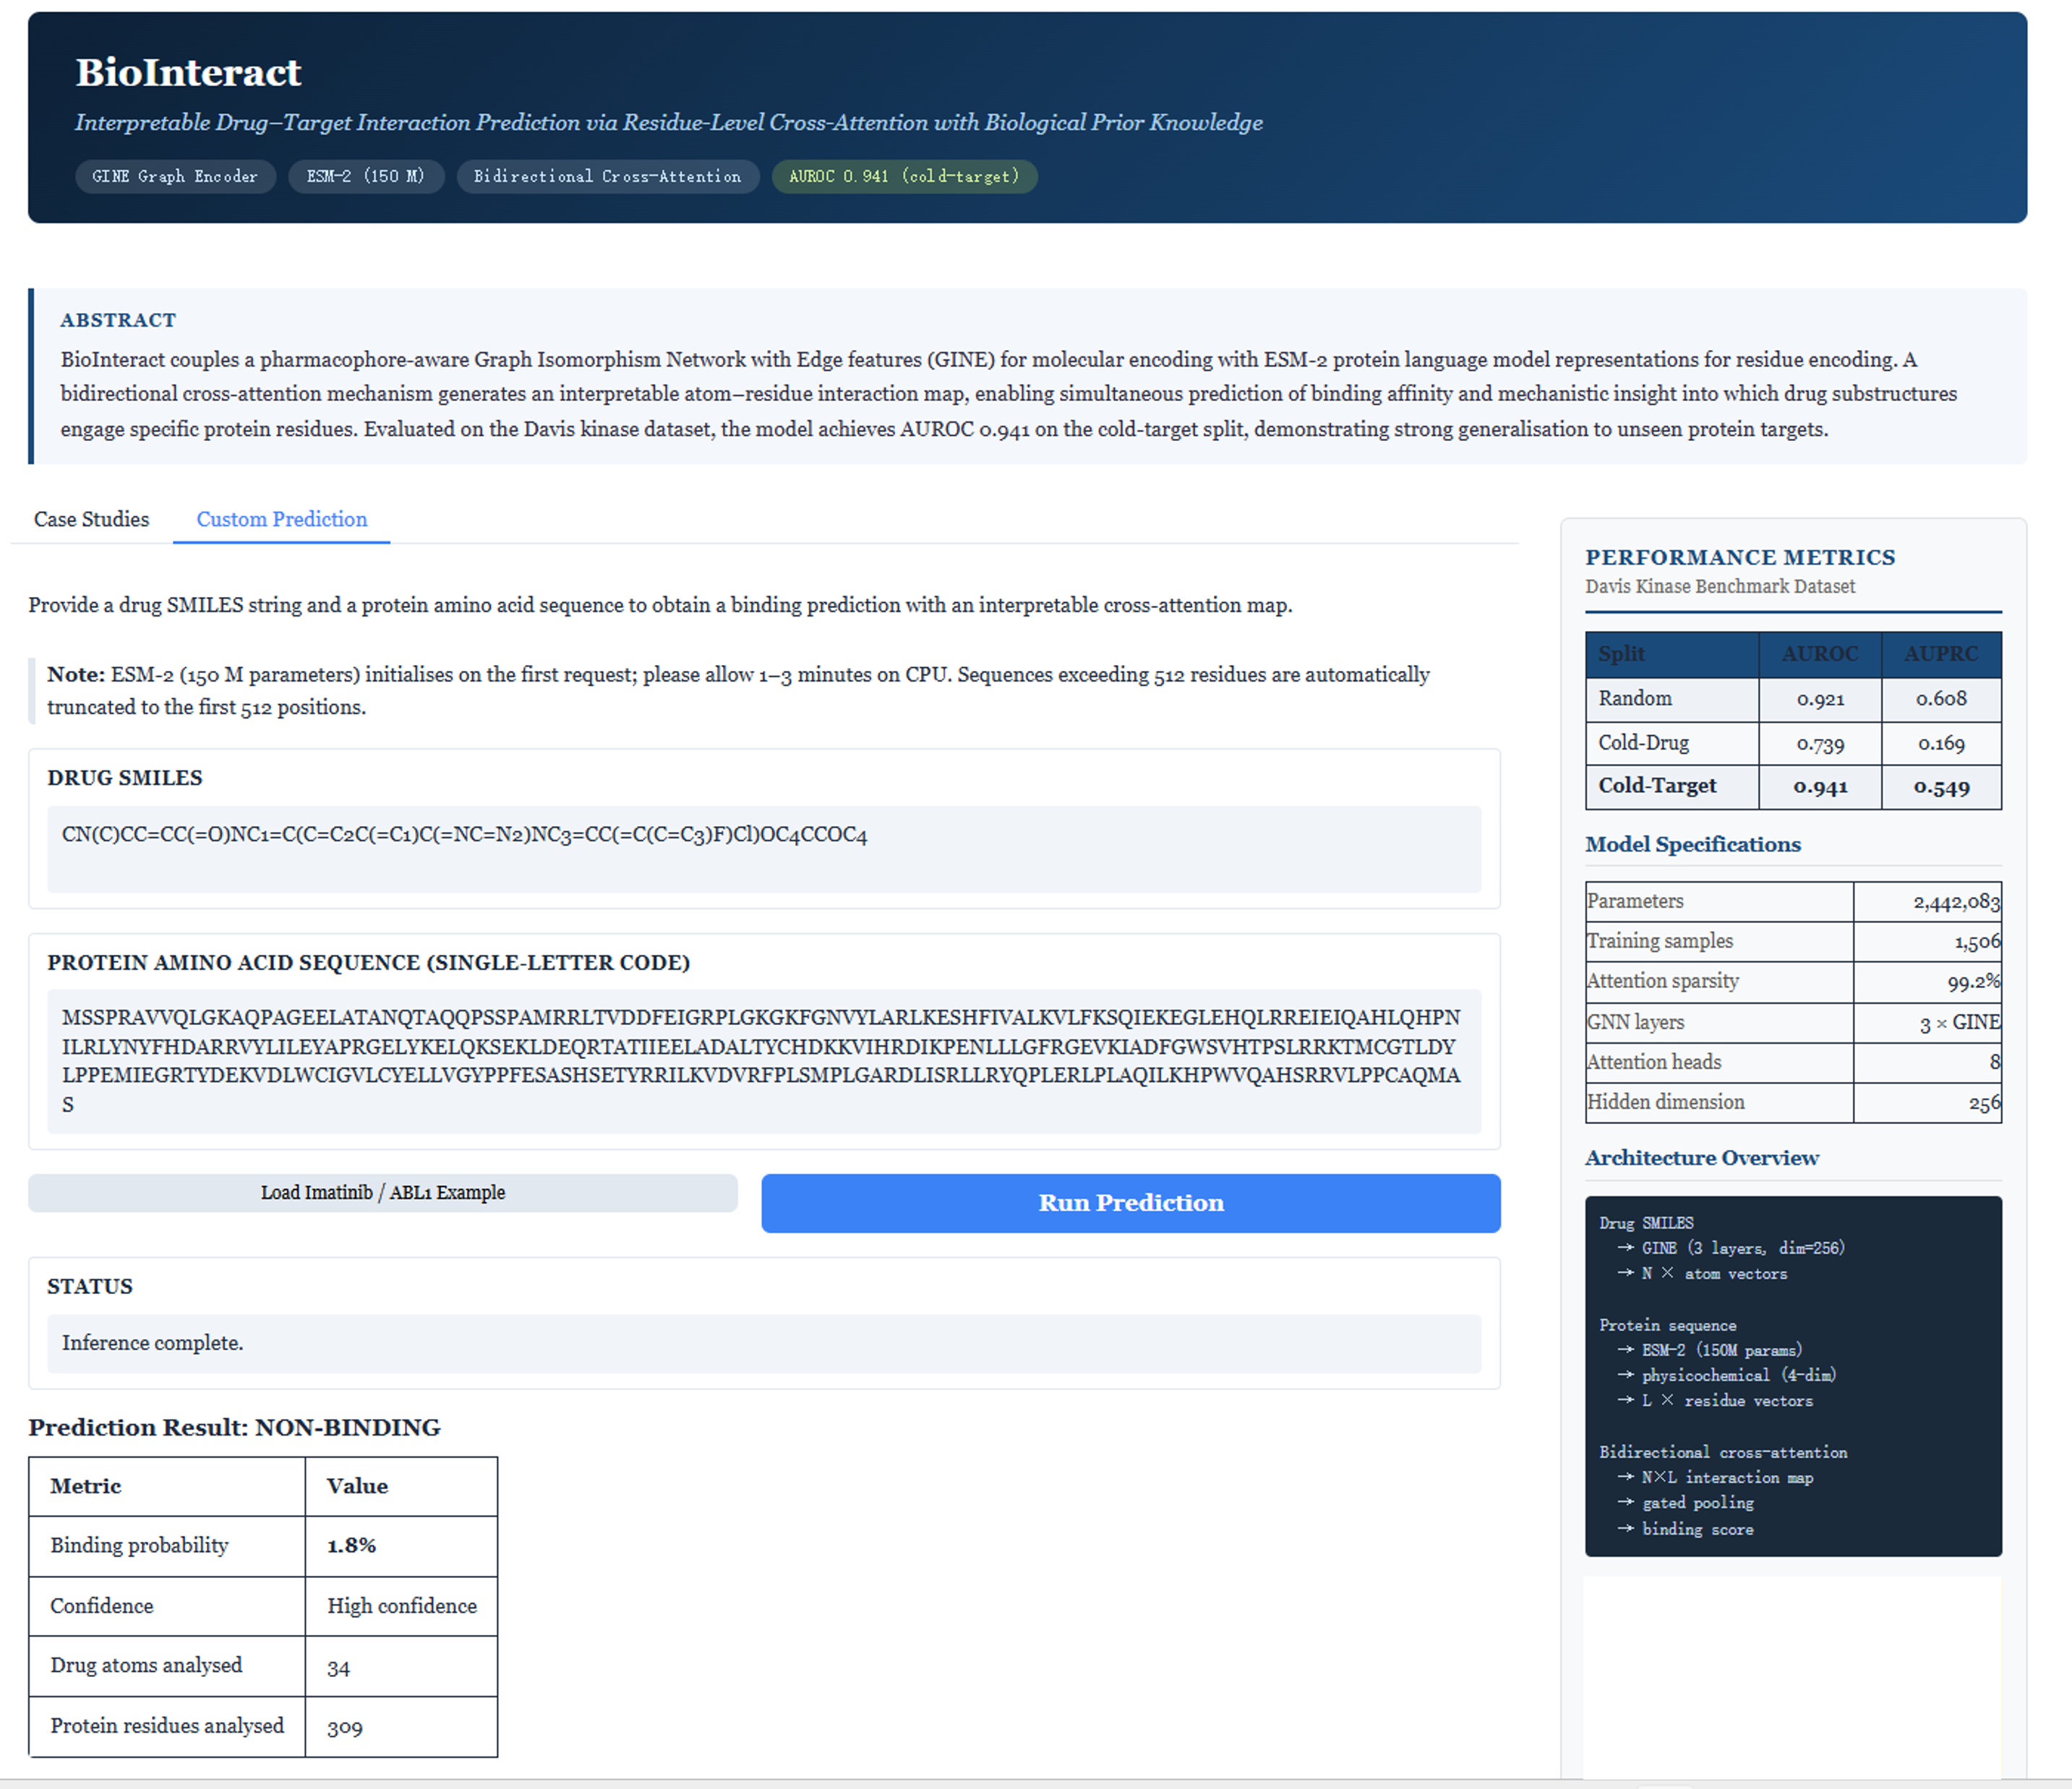
\includegraphics[width=\linewidth]{figures/WEB.png}
  \caption{\textbf{BioInteract interactive web server.}
    Screenshot of the publicly accessible interface at
    \url{https://huggingface.co/spaces/AI4deeperScience/BioInteract}.
    Users enter a drug SMILES string and protein amino acid sequence (\textit{left})
    and receive the binding probability together with a residue-level
    cross-attention heat map and ranked hotspot list (\textit{right}).
    No software installation is required.}
  \label{fig:webserver}
\end{figure}

BioInteract represents a step toward AI-assisted drug discovery in which
predictions are not only accurate but also \emph{trustworthy}, furnishing the
mechanistic rationale essential for informed molecular design.  Interpretable DTI
prediction, grounded in domain knowledge and evaluated against biochemical
reality, will be indispensable for the responsible integration of AI into
molecular discovery workflows.

%%====================================================================
\section*{Acknowledgements}
%%====================================================================

The authors thank Meta AI Research for providing the ESM-2 pretrained protein
language model and the RDKit developers for maintaining the open-source
cheminformatics toolkit.

%%====================================================================
\section*{Supporting Information}
%%====================================================================

The Supporting Information contains: complete model hyperparameters and
featurisation details (Tables~S1--S3); computational efficiency benchmarks
(Table~S4); dataset and split statistics with exact per-split metrics
(Tables~S5--S7); baseline method architectural summary (Table~S8);
full atom featurisation specification (Table~S9); detailed case-study residue
attention rankings for all ten drug--target pairs (Tables~S11--S14);
pairwise attention correlation matrix across ABL1 resistance mutants
(Table~S15); extended pharmacophore comparison across targets (Table~S16);
and complete model parameter counts (Table~S17).
This material is available free of charge.

%%====================================================================
\section*{Data Availability}
%%====================================================================

All data used in this study are publicly available. The Davis kinase inhibitor
dataset used for model training and evaluation is available from the original
publication.\cite{davis2011comprehensive} The BioInteract source code,
pretrained model weights, and figure-generation scripts are available at
\url{https://github.com/Liubo-520/bio-intelligence}. An interactive web
server for drug--target prediction and attention-map visualisation is available
at \url{https://huggingface.co/spaces/AI4deeperScience/BioInteract}.

%%====================================================================
\section*{Author Contributions}
%%====================================================================

\textbf{Shengnan Wang}: Conceptualisation, Methodology, Software, Formal
analysis, Writing -- original draft. \\
\textbf{Qi Zhang}: Methodology, Validation, Data curation, Visualisation,
Writing -- original draft. \\
\textbf{Xucheng Liu}: Investigation, Validation, Data curation. \\
\textbf{Zixuan Wang}: Software, Investigation, Data curation. \\
\textbf{Jiangke Cheng}: Resources, Validation, Visualisation. \\
\textbf{Zhi Huang}: Supervision, Writing -- review \& editing, Funding
acquisition, Corresponding author.

\vspace{0.5em}
\noindent S.\,Wang and Q.\,Zhang contributed equally to this work.
%%====================================================================

% Author A: Conceptualisation, Methodology, Software, Formal analysis, Writing -- original draft. \\
% Author B: Methodology, Validation, Data curation, Visualisation, Writing -- original draft. \\
% Author C: Investigation, Validation, Data curation. \\
% Author D: Software, Investigation, Data curation. \\
% Author E: Resources, Validation, Visualisation. \\
% Author F: Supervision, Writing -- review \& editing, Funding acquisition.

% \vspace{0.5em}
% \noindent Author A and Author B contributed equally to this work.
%%====================================================================
\section*{Declaration of Competing Interests}
%%====================================================================

The authors declare no competing interests.

\section*{Funding}

This work was supported by the Sichuan Provincial Key Laboratory for Development and Utilization of Characteristic Horticultural Biological Resources under Grant TSYY202502. The funder had no role in study design, data collection and analysis, decision to publish, or preparation of the manuscript.

\bibliography{sample}
\end{document}
